\documentclass[preprint,12pt, sort&compress]{elsarticle}

%% Use the option review to obtain double line spacing
%% \documentclass[authoryear,preprint,review,12pt]{elsarticle}

%% Use the options 1p,twocolumn; 3p; 3p,twocolumn; 5p; or 5p,twocolumn
%% for a journal layout:
%% \documentclass[final,1p,times]{elsarticle}
%% \documentclass[final,1p,times,twocolumn]{elsarticle}
%% \documentclass[final,3p,times]{elsarticle}
%% \documentclass[final,3p,times,twocolumn]{elsarticle}
%% \documentclass[final,5p,times]{elsarticle}
%% \documentclass[final,5p,times,twocolumn]{elsarticle}

%% For including figures, graphicx.sty has been loaded in
%% elsarticle.cls. If you prefer to use the old commands
%% please give \usepackage{epsfig}

%% The amssymb package provides various useful mathematical symbols
\usepackage{amsmath, amssymb}
\usepackage{makecell} %to have cells on multiple lines in tables
\usepackage{booktabs} % use \toprule, \midrule, \bottomrule in tables
\usepackage{changepage}
\usepackage{hyperref}
\usepackage{comment}
%% The lineno packages adds line numbers. Start line numbering with
%% \begin{linenumbers}, end it with \end{linenumbers}. Or switch it on
%% for the whole article with \linenumbers.
\usepackage{lineno}
\usepackage{color}

\graphicspath{{../../../Pictures/}}
\linenumbers

% CUSTOM DEFINITIONS

\newcommand{\bd}[1]{\boldsymbol{#1}}
\newcommand{\x}[1][]{\bd{x_{#1}}}
\newcommand{\R}[1][]{\mathcal{R}^{#1}}
\newcommand{\red}[1]{\textcolor{red}{#1}}




\journal{Energy and Buildings}

\begin{document}

\begin{frontmatter}

%% Title, authors and addresses

%% use the tnoteref command within \title for footnotes;
%% use the tnotetext command for theassociated footnote;
%% use the fnref command within \author or \address for footnotes;
%% use the fntext command for theassociated footnote;
%% use the corref command within \author for corresponding author footnotes;
%% use the cortext command for theassociated footnote;
%% use the ead command for the email address,
%% and the form \ead[url] for the home page:
%% \title{Title\tnoteref{label1}}
%% \tnotetext[label1]{}
%% \author{Name\corref{cor1}\fnref{label2}}
%% \ead{email address}
%% \ead[url]{home page}
%% \fntext[label2]{}
%% \cortext[cor1]{}
%% \affiliation{organization={},
%%             addressline={},
%%             city={},
%%             postcode={},
%%             state={},
%%             country={}}
%% \fntext[label3]{}

\title{Bayesian Uncertainty Quantification and Emulation of Building Energy Models: a Tutorial}

%% use optional labels to link authors explicitly to addresses:
%% \author[label1,label2]{}
%% \affiliation[label1]{organization={},
%%             addressline={},
%%             city={},
%%             postcode={},
%%             state={},
%%             country={}}
%%
%% \affiliation[label2]{organization={},
%%             addressline={},
%%             city={},
%%             postcode={},
%%             state={},
%%             country={}}

\author[1]{Dario Domingo\corref{cor1}}
\ead{dario.domingo@durham.ac.uk}
\author[2]{Mohammad Royapoor}
\author[1]{Hailiang Du}
\author[1]{Michael Goldstein}


\affiliation[1]{organization={Department of Mathematical Sciences, Durham University},
            addressline={Stockton Road}, 
            city={Durham},
            postcode={DH13LE}, 
            country={UK}}

\affiliation[2]{organization={Mohammad, please fill the affiliation},%Department and Organization
            addressline={}, 
            city={},
            postcode={}, 
            country={}}

\cortext[cor1]{Corresponding author}
\begin{abstract}
Correct calibration of building energy models is crucial to ensure that these can be reliably used to make predictions and inform design decisions. This work provides guidance and methodological steps for a systematic treatment of uncertainty before and during calibration. %, within a Bayes linear framework. 
We introduce emulation, a Bayesian technique to build a fast statistical surrogate of the model. The emulator’s speed allows to explore the model’s parameter space extensively in short timescales. The emulator’s predictions, alongside several quantified uncertainties, are then used to sequentially rule out model parameter configurations which are highly implausible to replicate the observed data. This procedure is known as History Matching (HM) and has been successfully employed even in high dimensions and with slow simulators. A package for its implementation is referenced. We discuss and illustrate HM on an example of a building energy model, where both energy consumption and temperature data are matched. The results show that only 0.3\% of the model input space leads to outputs that can match the observed energy consumption. The percentage reduces to 0.01\% if temperature constraints are also accounted for. The example shows the efficiency of HM to locate the small region where model outputs and observations can match, and therefore its ability to deliver models that lead to more robust decision support.
\end{abstract}

\begin{keyword}
%% keywords here, in the form: keyword \sep keyword
Uncertainty \sep Model Discrepancy \sep Building Energy Models \sep History matching.

%% PACS codes here, in the form: \PACS code \sep code

%% MSC codes here, in the form: \MSC code \sep code
%% or \MSC[2008] code \sep code (2000 is the default)

\end{keyword}

\end{frontmatter}

%%\linenumbers

%%%%%%%%%%%%%%%%%%%%%%%%%%%%%%%%%%
%%%%%%%%%%%%%%%%%%%%%%%%%%%%%%%%%%
%%%%%%%%%%%%%%%%%%%%%%%%%%%%%%%%%%

\section{Introduction}
\label{Sec_Intro}

Up to 40\% of primary energy use globally is attributed to buildings. Given the global decarbonisation efforts, accurate characterisation of building energy has become a key tool to enable optimal design, retrofit and investment decisions.  

In order to produce high-quality modelling results that acknowledge modelling limitations, full treatment of uncertainty becomes essential. This has driven an accelerated trend in model uncertainty research and performance gap analysis. A recent article has reported that a large proportion of the building modelling community lacks essential knowledge on what the most fundamental parameter inputs for buildings are and how these impact model predictions \cite{imam2017}. This knowledge gap has major consequences, as retrofit strategies are mostly derived in consultation with building energy models. As such, techno-economic benefits of proposed solutions can be misleading. In addition to this, future buildings are expected to become more responsive to other civic activities (i.e. power generation and storage, transport, etc.)\cite{royapoor2018}. Therefore imminent horizons require aggregated energy data at district and potentially city level, where accuracy and treatment of uncertainty are invaluable tools for decision makers at all levels.

A preliminary step to support model-based decisions is model calibration. Calibration is the process through which values of the model parameters are chosen, so that model outputs replicate observations within prescribed tolerances. Classically, this is performed by running the model multiple times, for different values of the parameters. Hence, for each simulation, one or more measures of the discrepancy between the corresponding output and the observed data are evaluated. In the context of building energy consumption, ASHRAE guidelines \cite{ashrae2002} are often followed \cite{royapoor2015, hou2021} to identify error thresholds below which the discrepancy can be considered sufficiently small. 

The main challenge of this approach is that the number of simulations needed to cover uniformly the model’s parameter space grows exponentially with increasing parameter dimensions. To meet the computational challenges involved, a new area of Bayesian statistics has arisen, namely emulation \cite{goldstein2017, kennedy2001, ohagan2006tutorial, craig2001}, part of the wider field of uncertainty quantification (UQ) of computer models. 

An emulator is a statistical surrogate of the simulator, providing predictions of the simulator’s outputs at inputs for which the original model has never been evaluated. The emulator can be built and validated on a personal device. It is instantaneous to run and therefore allows to predict the model results for a very large number of inputs. Moreover, it quantifies the uncertainty associated with such predictions. This explains the success of emulation in a wide range of fields where complex computer models are used, including but not limited to climate \cite{edwards2021} and energy price projections \cite{wilson2018}, epidemiology \cite{andrianakis2015}, hydrocarbon reservoirs \cite{craig1997} and galaxy formation \cite{vernon2010galaxy}.

Emulation is developed under Bayesian principles, arguably the most natural framework to deal with uncertainties. In the context of calibration, key uncertainties that are often overlooked are: i) the ability of the model to simulate the process of interest (for example, building energy consumption); ii) and the intrinsic accuracy of the observations used to calibrate the model. To deal coherently with these and other sources of uncertainty, we propose the use of so-called implausibility measures to compare model (or emulated) outputs and observations.

Implausibility measures have been employed in the contexts of reconstruction of ice sheet shapes \cite{domingo2020}, gene evaluation \cite{vernon2018gene}, galaxy formation \cite{vernon2010galaxy} and more, within a process known as History Matching (HM). The process sequentially removes regions of the input space deemed implausible to produce outputs which match the observations. However, in contrast to classical approaches in building energy model calibration, it does so in light of quantified uncertainties affecting various components of the system. 

This work is aimed at researchers in the energy community, who are keen to make their model-based inference more robust, by operating in a framework that recognises and accounts for unavoidable sources of uncertainty. The statistical framework is illustrated on an example study of a single-house energy model, where model parameters are sought that simultaneously match energy and environmental features. A link to an R package is provided, which allows the researcher to implement the proposed methodology within their own research.

This work is organised as follows. Section~\ref{Sec_Uncertainty} discusses key sources of uncertainty in computer model-based inference, particularly in the context of building energy models. Limitations of current approaches in this field are also outlined. Section~\ref{Sec_Methods} illustrates the proposed methodology: from emulation to implausibility measures and HM. Section~\ref{Sec_Example} gives details of the building energy model and field data used in our case study. Results on the example study are illustrated in Section~\ref{Sec_Results}, where we also discuss approaches to scenarios that may be encountered in other case studies. Section~\ref{Sec_Discussion} concludes the article with discussions and work extensions.

%%%%%%%%%%%%%%%%%%%%%%%%%%%%%%%%%%
%%%%%%%%%%%%%%%%%%%%%%%%%%%%%%%%%%
%%%%%%%%%%%%%%%%%%%%%%%%%%%%%%%%%%

\section{Uncertainty Sources in Building Energy Models}
\label{Sec_Uncertainty}

%%%%%%%%%%%%%%%%%%%%%%%%%%%%%%%%%%

\subsection{Calibration under Uncertainty}

Calibration is a crucial topic not just in energy, but in a variety of scientific disciplines. It refers to the process by which the parameters of a computer model are identified so that model outputs match observed data. Mathematically, the model (or simulator) can be seen as a function $f$, with input $\x$ containing the list of model parameters of interest, and returning $f(\x)$ as output. If we call $z$ the observed data we want to match, the calibration task can be phrased as finding the input(s) $\x$ so that $f(\x)$ is “close enough” to $z$. In practical applications, we often have a sequence of observations to match (and correspondingly a sequence of model outputs), rather than a single observation.

Proximity between simulations and observations should be assessed upon consideration of all sources of uncertainty that affect the system. While an exhaustive list of such sources is problem-dependent and challenging to specify in its entirety \cite{kennedy2001}, two sources of uncertainty usually play a prominent role in energy system modelling and beyond:
\begin{enumerate}
\item \emph{Model Discrepancy (MD)}. Due to unavoidable modelling assumptions and numerical approximations, the output  simulated by a model $f$ at an input $\x$ will be different from the value that would be observed in the real world under the same physical conditions represented by $\x$. This difference is referred to as model discrepancy.
\item \emph{Observational Error (OE)}. It is a source of uncertainty intrinsic to all physical measurements, with a magnitude that depends on the employed measurement device
\end{enumerate}

Accounting for these two uncertainty sources is crucial to assess whether a model has been successfully calibrated against observed data, and to make sure that robust inference can be drawn from the calibrated model predictions.

%%%%%%%%%%%%%%%%%%%%%%%%%%%%%%%%%%

\subsection{Model Discrepancy in Building Energy Systems}
\label{Subsec_MD_Energy}
This section highlights sources of model discrepancy typical of building energy models, arising from a  wide range of assumptions that analysts need to make

\subsubsection{Building Thermal Properties}
In a study of two office buildings in Australia \cite{daly2014}, cooling set-points, lighting power density, ICT infrastructure and its schedule were found to impact the predictions of energy models the most. In other words, model predictions were found to be particularly sensitive to small changes in these parameters. 
Secondly, a major source of model discrepancy concerns the fabric thermophysical properties, the fabric composition (i.e., non-homogeneity, moisture content affecting thermal conductivity, etc.), as well as surface properties (radiative or convective characteristics). Most notably, the hypothesis of mono-dimensionality of heat flow - which is fundamental to thermal resistance (U-value) calculations in ISO 6946:2007 \textcolor{red}{(Mohammed, can you please provide the bibtex references for SO 6946:2007 and ISO 9869-1:2014, corresponding to references number 5 and 8 of the word document?}, ISO 9869-1:2014, CIBSE and ASHRAE [5-8] \textcolor{red}{(same for CIBSE an ASHRAE, references number 6 and 7. I can't uniquely locate them on google scholar nor elsewhere.)  (Maybe check, whether the ASHRAE reference - number 7 - can be replaced by my current number 3?)} – remains a major simplification. In solid bodies, heat travels in a diffused and 3-dimensional manner which no building energy modelling platform replicates. 
Thirdly, for existing structures, notable differences in thermal property measurements exist across seemingly uniform building envelops \cite{rasooli2016, deconinck2016, meng2015, ficco2015}. These divergences are then compounded further given that they are used in U-value calculations (either semi-stationary or dynamic) that each produce a slightly different outcome \cite{deconinck2016} (disagreements of up to 393\% are reported between measured and calculated figures \cite{rasooli2016}). While traditional solid masonry walls \cite{gaspar2016, desogus2011} and floors \cite{hoffmann2017} have been found to perform better than model calculations, actual composite walls are reported to perform worse than models suggest. A. Marshall et al. found CIBSE model U-Values for brick walls, ceilings and doors to over-predict performance by 30.3\%, 15.5\% and 9.9\% respectively while calculated window properties showed much better matches with measured figures \cite{marshall2017}. A study of 57 properties found that while variations between similar wall types and even within the same dwelling’s walls existed, 44\% of walls performed better than CIBSE calculations, 42\% were within acceptable bounds and only 14\% of sampled walls performed worse than calculations suggest \cite{baker2011}, however measured and calculated floor U-values were found to be in good agreement. In summary difficulties in identifying the composite material and their density and moisture content, internal and external air velocities, fabric non-homogeneity and cumbersome nature of in-situ fabric studies are notable reasons behind fabric U-value uncertainties. 

\subsubsection{Weather and Occupant Activity}
The micro-climate around a building is by its nature random, with a particular set of conditions never repeating itself over the building’s lifetime. It is affected by wind speed and direction, solar irradiance both outside and within the building, external temperature and humidity, cloud cover and ground albedo, atmospheric pressure. These all interact in close-to-chaotic manner to dictate a micro-climate, which is then represented in a simplified annual weather file for most energy simulations. Weather files are normally extracted from decades of actual data (e.g. using Finkelstein-Schafer method) but remain a major source of energy simulation uncertainty for the following reasons: i) building energy performance is affected by future rather than past weather; ii) a single weather file can hardly represent all meteorological conditions; iii) most weather files are not measured at the site but at a nearby meteorological station (often exposed airports), leading to inadequate representation of urban heat island and sheltering effects \cite{yassaghi2019}.

Second to micro-climate, the occupant behaviour is drastically simplified to inform the current generation of simulation tools. Temporal schedules usually describe the variations in occupant-related activities in a homogenous and deterministic form. More accurate representations of the occupant’s dynamic interaction with the building remain an active area of research. Advances in pervasive sensing and data collection have enabled better understanding of occupant presence and movements. Insights from improved monitoring have informed two categories of occupant representation: implicit and explicit models that predict stochastic occupant interventions with windows, ICT and HVAC. Improvements are gained by seeking to understand the underlying logic behind occupant interaction with its surrounding at a behavioural level (explicit method) \cite{hong2016}. Challenges remain in adequately detailed monitoring of occupant behaviour, the integration of future occupant behaviour into simulation models and validation of the approach against longitudinal field studies. W. Tian et al. \cite{tian2018} note the need for further research to provide clear guidance not only to characterise stochasticity but also on the number of samples required to arrive at acceptable statistical power in building energy analysis \cite{tian2018}. This remains a priority particularly if post pandemic workplace attendance continues to evolve under a hybrid working regime.

%%%%%%%%%%%%%%%%%%%%%%%%%%%%%%%%%%

\subsection{Limitations of Current Calibration Approaches in Building Energy Models}
\label{Subsec_Limitations}

None of the approximations and assumptions discussed in Section~\ref{Subsec_MD_Energy} undermines the validity of a model. However, awareness of similar assumptions and approximations is key to quantify the discrepancies induced when comparing model outputs and real-world observations.

In the context of building energy models, ASHRAE guidelines \cite{ashrae2002} are often followed to assess whether a model has been successfully calibrated against observed data \cite{royapoor2015, hou2021}. The guidelines make use of the following discrepancy measures between a sequence of N simulated model outputs $S_i$, and a corresponding sequence of observations $M_i$:
\begin{align}
 \text{MBE}             &= \frac{\sum(M_i - S_i)}{\sum M_i} \label{eqn_MBE}\\[1ex]
 \text{CV(RMSE)}  &= \frac{\sqrt{\frac{1}{N} \sum(M_i - S_i)^2}}{\frac{1}{N} \sum M_i} \label{eqn_CVRMSE}
\end{align}
The model is considered calibrated if the relevant condition of the following two is met:
\begin{enumerate}[(a)]
\item Hourly measurements: $-10\% \leq \text{MBE} \leq 10\%$ and $\text{CV(RMSE)} \leq 30\%$. \label{criterion_hourly}
\item Monthly measurements:  $-5\% \leq \text{MBE} \leq  5\%$  and $\text{CV(RMSE)} \leq 15\%$.\label{criterion_monthly}
\end{enumerate}

While the above criteria are easy to check, their use to assess model calibration presents some limitations. Firstly, acceptance thresholds are independent of the level of accuracy to which measurements are available, and of the level of discrepancy between the model and reality. Moreover, formulas \eqref{eqn_MBE} and \eqref{eqn_CVRMSE} are not applicable to some of the physical quantities for which model outputs and observations may be available. 

Indeed, the two formulas measure the magnitude of the (average) bias and root mean square error of the sequence $M_i-S_i$, relative to the (average) measured value. This is meaningful for any quantity intrinsically defined on a positive scale, such as energy consumption, but becomes less meaningful for other quantities, such as temperature. Here, using different units (\textit{e.g.}, degrees Celsius or Kelvin) leads to seemingly different results. In reality, only Kelvin should be used, but in this case criteria \eqref{criterion_hourly} and \eqref{criterion_monthly} would be easily fulfilled due to the large denominator in \eqref{eqn_MBE} and \eqref{eqn_CVRMSE}.  

In Section~\ref{Sec_Methods}, we propose a statistical framework which overcomes these limitations. The framework makes it easy to account for recognised uncertainties when model and data are compared and it is applicable to any quantity of interest (and, in fact, to several quantities simultaneously). Moreover, thanks to the use of emulators, the framework can explore the model response at millions/billions of inputs, in a fraction of the time required for physics-based models to generate output. 


%%%%%%%%%%%%%%%%%%%%%%%%%%%%%%%%%%
%%%%%%%%%%%%%%%%%%%%%%%%%%%%%%%%%%
%%%%%%%%%%%%%%%%%%%%%%%%%%%%%%%%%%


\section{Methodology}
\label{Sec_Methods}

This section presents statistical methods to quantify and include different sources of uncertainty during model calibration. The overall process we illustrate is referred to as History Matching (HM). The name was first used within a study on hydrocarbon reservoirs \cite{craig1997} and indicates the attempt to “replicate history” i.e., to produce model outputs that match historical data. Since then, its statistical principles and methods have been successfully applied to a variety of fields (climate \cite{domingo2020}, biology \cite{coveney2018}, epidemiology \cite{andrianakis2015}, cosmology \cite{vernon2010galaxy} and more). However, in energy systems there has been little to no application that are reported in the literature. 

In this section we discuss the tools and statistical principles underlying HM, illustrate the procedures and provide statistical packages to implement it. We hope that our exposition, and the following illustration to a building energy example study, will promote its uptake within the energy community, and enable a robust treatment of uncertainty in calibration of computer models.

The HM procedure sequentially rules out regions of the model’s input space where, in light of all quantified uncertainties, model outputs cannot match observed data. Emulators and implausibility measures are the two key tools used to accomplish the task as follows:
\begin{itemize}
\item Emulators allow to predict the model output at choices of input parameters where the model has never been run, quantifying the uncertainty of the prediction. Given their speed, emulators can be used to explore the model parameter space thoroughly, even in higher dimensions.
\item Implausibility measures quantify the distance between model outputs and observations, in light of different sources of uncertainty.
\end{itemize}

Section~\ref{Subsec_Emulators} provides an overview of emulation, in simple but comprehensive terms. Sections~\ref{Subsec_MD}--\ref{Subsec_HM} then formalise the concepts of model discrepancy and measurement error, introduce implausibility measures, and illustrate the overall HM procedure, respectively.

%%%%%%%%%%%%%%%%%%%%%%%%%%%%%%%%%%

\subsection{Bayes Linear Emulators as Fast Model Surrogates}\label{Subsec_Emulators}

Evaluating the model’s response across its input space, and comparing its outputs to observations, is a key part of calibration. However, running a number of simulations that thoroughly cover the parameter space proves unfeasible due to time and computational constraints. Emulators can be employed to overcome this issue.

An emulator is a statistical surrogate of the model, predicting the model’s outputs at inputs where the model has never been run. Emulators’ most evident advantages are speed and low computational requirements. A nominal measure of this speed is that predictions of the output of interest at thousands of different inputs can be obtained in one second on a personal laptop. Moreover, the emulator prediction is accompanied by a precise uncertainty statement of its accuracy, which lays the basis for model uncertainty analysis.

In this work we employ Bayes linear emulators (BLEs) to replicate the behaviour of the example-study building energy model (see section~\ref{Sec_Example}). One emulator is built for each output of interest. In this section, we give a brief overview of the choices behind the construction of a BLE, referring the reader to \cite{goldstein2017, vernon2010galaxy} for further details. The interested reader is also referred to \cite{BLS2007} for a much more in-depth treatment of Bayes Linear principles. 

We use the following form for $f(\x)$, the output of the computer model at input $\x$:
\begin{equation}\label{eqn_emulator}
f(\x) = \sum_j \beta_j g_j(\x) + u(\x)\,.
\end{equation}

Equation~\eqref{eqn_emulator} is made of two terms. The first one is a regression component: it uses a linear combination of known functions $g_j(\x)$ to model the global behaviour of $f$ across the input space. The second term, instead, is meant to capture the local fluctuations of $f$, once the main regression component has been accounted for. 

Now suppose that the model has been run at a sequence of inputs $\x[1], \dots, \x[n]$. Each $\x[i]$ is called a design point and we will denote the corresponding output by $y_i = f(\x[i])$. Then:
\begin{itemize}
\item The coefficient $\beta_j$ in equation~\eqref{eqn_emulator} can be estimated by fitting a linear regression model with predictors $g_j(\x)$ to the known pairs $(\x[i], y_i)$.
\item Values of the residual process $u(\x)$ will then be known at each design point: $u(\x[i])=u_i$. These values will approximately oscillate around $0$, with local patterns that the regression term has not been able to detect. We predict values of $u(\x)$ via a BLE.
\end{itemize}
The idea to this last point is to model $u(\cdot)$ as a stochastic process, specifying a prior mean and covariance structure for it. In the Bayes linear framework, these are then adjusted to the observed values $u_i$ at $\x[i]$, yielding an adjusted mean prediction and uncertainty statement for $u(\x)$, at any $\x$.

The prior specifications we make for $u$ are as follows. We assume $u(\x)$ to have mean zero at all inputs $\x$ and we use a stationary kernel to model the covariance between the value of $u$ at any two inputs $\x$ and $\widetilde{\x}$. A stationary kernel is one for which the above covariance only depends on the difference $\x - \widetilde{\x}$. For common choices in emulation see Section 4.2.1 of \cite{Rasmussen}. In this work, we use the squared exponential kernel, leading to the following formula:
\begin{equation}\label{eqn_kernel}
\text{Cov}[u(\x), u(\widetilde{\x})] = \sigma_u^2 \, \exp \left( - \sum_k \left(\frac{x_k - \widetilde{x}_k}{d_k}\right)^2 \right)
\end{equation}
The subscript $k$ in $x_k$ and $\widetilde{x}_k$ denotes the $k^{th}$ component of the two inputs, \textit{i.e.}, the $k^{th}$ model parameter. The positive coefficient $d_k$ (called correlation length, or length scale) measures the strength of correlation in outputs when the $k^{th}$ parameter is modified. Finally, the coefficient $\sigma_u^2$ denotes the prior variance of $u(\x)$ at all inputs $\x$.

Expression~\eqref{eqn_kernel} has been written in terms of all components of the input vector $\x$. However, just some of the parameters often prove relevant to explain the great majority of the variability in $u$. We call these active parameters and, in practice, only use them in expression~\eqref{eqn_kernel}. The small variability left in $u$, due to the inactive parameters, is modelled as uncorrelated noise with constant variance $\nu^2$.

Notice that no distribution has been assumed for the process $u$. Within the Bayes linear framework, we only need to specify mean and covariance, as above. These mean and covariance are then adjusted to the values $u(\x[i])=u_i$, yielding an adjusted mean and variance for the value of $u(\x)$ at any $\x$. Details of the adjusted mean and covariance formulas can be found for example in \cite{goldstein2017, vernon2010galaxy, BLS2007}.
The above should however be sufficient to clarify the setting within which a BLE is built, and the decisions that need to be made. In particular, these are: the predictors $g_j$ of the regression term; the variances $\sigma_u^2$ and $\nu^2$; the active parameters; the correlation lengths $d_k$. 

Although – put strictly - the above procedure builds a BLE for the “residual” process $u$, once the regression prediction at $\x$ is added, an overall prediction for $f(\x)$ is obtained. Ultimately, this is the focus of interest. For this reason, in the following the term emulator will refer to the overall emulator of $f$. At any input $\x$, this provides a prediction $\hat{f}(\x)$ of the unknown value $f(\x)$, and a standard deviation $\hat{s}(\x)$ quantifying the potential error of such prediction.

%%%%%%%%%%%%%%%%%%%%%%%%%%%%%%%%%%

\subsection{Model Discrepancy and Observational Errors}\label{Subsec_MD}
The concepts of model discrepancy (MD) and observational error (OE) are relevant to any uncertainty analysis linking computer simulations and measurements \cite{vernon2010galaxy, vernon2018gene, craig1997, domingo2020}.
In this section we formalise them using a general framework. To relate the notation to the context of building energy models, the reader may think of: $\x$ as a set of model parameters; $f(\x)$ as the simulated consumption in the building under parameters $\x$; $y$ as the actual energy consumed in the building; $z$ as the (imperfect) meter reading reporting the consumed energy. 

Following\cite{goldstein2017}, we assume that an appropriate choice of inputs exists, $\bd{x^*}$, that accurately represents the values of the system’s parameters. We then link the simulator output $f(\bd{x^*})$ at this parameters configuration and the real-world value y of the quantity being modelled, via the formula:
\begin{equation}\label{eqn_MD}
y = f(\bd{x^*}) + \varepsilon_{MD}\,,
\end{equation}
where the model discrepancy term $\varepsilon_{MD}$ accounts for the difference between the real and the simulated process. While the assumption is that just one quantity is being modelled, the same formulation can be considered if both $y$ and $f(\x)$ were vectors. 

The unobservable real-system value $y$ is usually estimated through a measurement $z$. We link these two quantities via the relationship:
\begin{equation}\label{eqn_OE}
y = z + e_{OE}\,,
\end{equation}
where the term $e_{OE}$ accounts for the observational error in the measurement.

The additive formulation in equations~\eqref{eqn_MD} and \eqref{eqn_OE} is a simple but efficient way to model MD and OE, which also makes statistical inference tractable. Information about the quantities $ \varepsilon_{MD}$ and $e_{OE}$ should in fact be sought in statistical form, rather than quantified as a single number.

Manufacturer guidelines are usually available to estimate the OE magnitude (e.g., up to $5\%$ of the measured value). Estimates of MD magnitude may be more challenging to obtain. However, the modeller’s knowledge of the assumptions and approximations used within the simulator, alongside literature research, usually provide guidance on the uncertainty effects of different assumptions and can therefore lead to an overall estimate of MD.

In the example study discussed in this work, we consider two different levels of MD ($10\%$ and $20\%$ of the emulated value of $f(\x)$), discussing how the choice affects the results (Section~\ref{Sec_Results}). For a more detailed treatment of MD, and the further distinction between internal and external MD, the reader is referred to \cite{goldstein2017}.

%%%%%%%%%%%%%%%%%%%%%%%%%%%%%%%%%%

\subsection{Implausibility Measures}\label{Subsec_IM}
Given a computer model $f$ of a physical system and measurements $z$ of the system, this section outlines how to measure the likelihood that an input $\x$ to the model well represents the system’s features. We do this by comparing $f(\x)$ and $z$. As we will see, acknowledging the involved uncertainties will naturally lead to measure implausibility as opposed to likelihood.

The setting is as follows. A series of observations $z_1, \dots, z_m$ of $m$ different quantities is available. Each quantity is modelled by the simulator: $f_j(\x)$ denotes the simulator prediction of quantity $j$ at input $\x$.  For instance, in the case of a building energy model, $z_j$ and $f_j$ may represent measured and predicted consumption in month $j$. To make the notation lighter, in the following we initially drop the index $j$, reintroducing it later where information from different measurements/model outputs will be aggregated. 

The construction of implausibility measures is based on the following reasoning. A choice of input parameters $\x$ well represents the hidden system's parameters (called $\bd{x^*}$ in Section~\ref{Subsec_MD}) if the following two quantities coincide:
\begin{enumerate}[i)]
\item \label{cond1} The value assumed by the real system under conditions $\x$ (eg, energy consumed under building parameters as in $\x$)
\item \label{cond2} The actual value y of the real system (eg, actual energy consumed in the building).
\end{enumerate}
None of the two quantities is available for general $\x$, but both can be estimated, respectively by $f(\x)$ (the model predicted consumption at $\x$) and $z$ (the measurement of $y$, such as a meter reading). 
%In the notation of Section\ref{Subsec_MD}, we can write \ref{cond1}) as $f(\x) + \varepsilon_{MD}$ and \ref{cond2}) as $z+e_{OE}$.

Hence, by comparing the difference $f(\x) -z$ to the tolerance allowed by MD and OE, 
we can establish whether the quantities in \ref{cond1}) and \ref{cond2}) may or may not be the same. This leads us to consider the following quantity:
\begin{equation}\label{eqn_IM_initial}
\frac{|f(\x) - z|}{\sqrt{\text{Var}(\varepsilon_{MD}) + \text{Var}(e_{OE}) }\,}
\end{equation}
High values of the the quantity above make the input $\x$ \emph{implausible} to match the unknown system features $\bd{x^*}$ having led to observe $z$.

Notice that expression~\eqref{eqn_IM_initial} requires knowledge of the simulated value $f(\x)$. In practice, this is rarely readily available. However, if an emulator of $f$ has been trained, the emulator prediction $\hat{f}(\x)$ can be used as estimate of $f(\x)$. To account for the substitution, the emulator variance ${\hat{s}(\x)}^2$ should be included in the denominator of~\eqref{eqn_IM_initial}. Therefore, reintroducing the index $j$ to indicate the particular output in question, we define:
\begin{equation}\label{eqn_IM}
I_j(\x) = \frac{|f_j(\x) - z_j|}{\sqrt{\text{Var}(\varepsilon_{MD}^j) + \text{Var}(e_{OE}^j) +  {\hat{s}_j(\x)}^2}\,}
\end{equation}
the implausibility measure of input $\x$, with respect to quantity $j$.
Finally, as overall measure of implausibility with respect to all the $m$ quantities under consideration, we define:
\begin{equation}\label{eqn_IM_overall}
I(\x) = \max_j I_j(\x)\,.
\end{equation}

The rationale behind the above definition is as follows. A high value of $I(\x)$ implies that at least one of the $I_j(\x)$ is high. In other words, the input $\x$ has led to an output $f_j(\x)$ that is highly incompatible with the observed value $z_j$, even after accounting for the involved sources of uncertainty (MD, OE, emulation). In this case, we say that the input $\x$ is \textit{implausible} to lead to a match. Vice versa, we call $\x$ \textit{non-implausible}, since the involved uncertainties make it possible for $\x$ to lead to a match between model outputs and observations.

The history matching algorithm, described in Section~\ref{Subsec_HM}, sequentially rules out all implausible inputs, identifying a final region where model outputs and observations can match in light of quantified uncertainties. 

%%%%%%%%%%%%%%%%%%%%%%%%%%%%%%%%%%

\subsection{History Matching: The Algorithm}\label{Subsec_HM}

History matching (HM) proceeds in waves. The procedure is illustrated below and summarised thereafter in a schematic algorithm.

In the first wave, some or all of the model outputs for which observations are available are emulated. The implausibility measure~\eqref{eqn_IM_overall} is computed across the space, and all inputs $\x$ for which $I(\x)$ exceeds a given threshold are discarded as implausible. The remaining region, comprising the currently “non-implausible” points, is usually referred to as the Not-Ruled-Out-Yet (NROY) region.

The process is repeated, in consecutive waves. Crucially, at any new wave, additional simulations are run within the current NROY region, before new emulators are trained and an additional fraction of the region is discarded as implausible. The procedure terminates when the NROY region does not shrink any further, or it has become empty (all inputs have been ruled out as implausible). 

The algorithm below summarises the steps. Comments on the procedure and guidance on some of the choices follow in Section~\ref{Subsec_HM_comments}.
\vspace{2ex}

\noindent
\underline{\it History Matching Algorithm}\\[1.5ex]
Choose a positive threshold T (guidance provided in Section~\ref{Subsec_HM_comments}). Define a sequence of NROY regions $\R[0]\supseteq \R[1]\supseteq \dots \R[k]\supseteq \R[k+1] \dots $ as follows:
\begin{enumerate}
\item 	Initial Step ($k=0$)
\begin{enumerate}
\item Let $\R[0]$ be the whole input space. Perform a sequence of model runs in $\R[0]$, and build emulators of some of the quantities for which observations are available.
\item Let $I^0$ be the implausibility measure in equation~\eqref{eqn_IM_overall}. Define the first NROY region as $\R[1] = \{ \x \in \R[0] \, : \,  I^0(\x)<T \}$.  
\end{enumerate}
\item 	Iterative Step ($k\geq1$)
\begin{enumerate}
\item 	Run additional simulations within $\R[k]$. Decide which outputs to emulate, and build emulators for them based on old and new runs within $\R[k]$. \label{point_iterative}
\item 	Compute the implausibility $I^k(\x)$ over $\R[k]$, and identify $\R[k+1]$ as $\R[k+1]=\{\x \in \R[k] \,:\, I^k(\x)<T \}$.
\end{enumerate}
\item Stop when $\R[k+1]=\R[k]$ or $\R[k+1]$ is empty.
\end{enumerate}
The flowchart in Fig.~\ref{Fig_FlowChart} illustrates the overall methodology. 

\begin{figure}
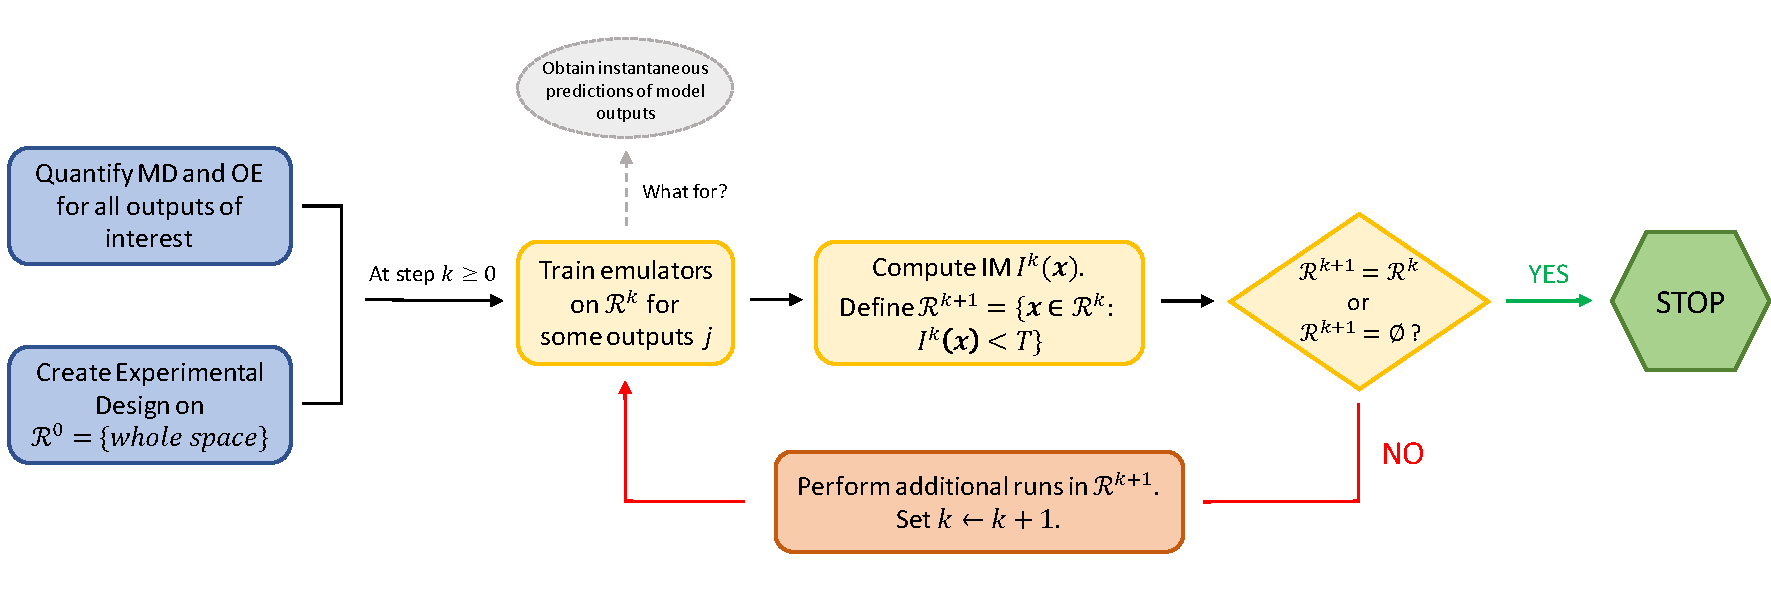
\includegraphics[width=\textwidth]{Pictures/Flow_Chart/FlowChart_Horizontal.pdf}
\caption{Flow chart illustrating the History Matching (HM) procedure. The initial steps (blue) consist in quantifying the main sources of uncertainty and designing a first set of runs over the whole space. The central part of the diagram (yellow) describes the steps of a typical wave, which aims to reduce the volume of the region comprising currently non-implausible inputs. Consecutive waves are repeated, till the region cannot be further reduced, or it is empty.}
\label{Fig_FlowChart}
\end{figure}

%%%%%%%%%%%%%%%%%%%%%%%%%%%%%%%%%%

\subsection{Comments on the Procedure and its Strengths in Handling Uncertainties}
\label{Subsec_HM_comments}

We comment here on some of the choices needed to perform HM and on the overall strengths of the procedure, particularly in handling uncertainties.

The choice of the threshold $T$ reflects how large an implausibility we are prepared to accept, before ruling out an input as implausible. A common choice is $T=3$, based on Pukelsheim’s $3\sigma$ rule \cite{3sigma}. See \cite{vernon2010galaxy} for more details. 
However, a larger threshold may be chosen if several quantities are being history-matched. Indeed, mainly due to emulation error, for each fixed output $j$ there is some small probability that $I_j(\x) > T$ even if $\x$ was the ``best'' input $\bd{x^*}$. This probability increases if we consider the event that \emph{at least} one $j$ leads to $I_j(\x)>T$, that is, the event $I(\x)>T$. Therefore, a larger threshold $T$ ensures that this probability of error is kept low.

As highlighted by point~(\ref{point_iterative}) of the algorithm, at each wave, only some of the model outputs are used to compute the implausibility measure. This is a key feature of HM. Especially in early waves, some of the outputs may be difficult to emulate over large parts of the space, typically because the model’s behaviour varies significantly across different input regions. As the search of non-implausible inputs is narrowed down to much smaller regions, outputs that were difficult to emulate may behave more uniformly within the region of interest. They can therefore be emulated precisely and included in the definition of $I(\x)$ to rule out further implausible regions. 

Also notice that, especially in earlier waves, not ruling out an input ($I(\x)\leq T$) does not suggest that the input leads to a match with the observations. Indeed, the implausibility of an input $\x$ may be low as a consequence of large emulator uncertainty (term $\hat s_j$ in equation~\eqref{eqn_IM}), rather than actual proximity between the emulated prediction and the observation. However, emulator uncertainty is typically reduced between waves, because the emulators are trained on smaller regions (where the simulator may behave more smoothly) and on more design points. Reducing emulator uncertainty leads to larger implausibilities and, therefore, to more inputs being identified as implausible. 

This is, in fact, the rationale behind proceeding in multiple waves and a key strength of HM. The decision of rejecting an output as implausible is taken in light of all quantified uncertainties at the given stage, including MD and OE. In this regard, notice that expression~\eqref{eqn_IM} can be easily adjusted to include additional sources of uncertainty in its denominator, whenever these are recognised and quantified in the problem in question. Moreover, by only involving differences and measurements of variability, implausibility measures can be computed for any quantity for which measurements are available, even if these are not measured on a positive scale (\textit{e.g.}, Celsius degrees for temperature). This marks a crucial difference with respect to formulas \eqref{eqn_MBE}~and~\eqref{eqn_CVRMSE}.

In most cases, one or two waves are enough to rule out as implausible a great percentage of the space. In fact, as shown in the example study of Section~\ref{Sec_Example}, one wave may even be enough to identify the final non-implausible region, if the emulator uncertainties are negligible with respect to MD and OE. More generally, however, multiple waves may be needed. In R, the hmer package \cite{hmer} can be used to implement emulation and HM. The package guides the researcher into multiple HM waves, by automatically suggesting a new design for each wave. %Due to the low time and computational resources needed for emulation, HM can be performed on a personal laptop. 

We conclude this section with a consideration. By designing model runs only where needed, HM allows the researcher to focus sequentially on the region of interest, while keeping the overall number of runs low. This is crucial in medium and high dimensions. In these cases, the region where a match is possible may only represent a tiny fraction of the original space. A more na\"ive yet not uncommon approach, where a number of simulations are run across the space and compatibility with observations is checked on these, would almost surely miss the region, even if the number of runs was very large. HM allows instead to identify the region precisely (even in high dimensions) thanks to the sequential “refocussing” procedure. 

The event where, at some wave, all inputs have been discarded as implausible, is possible and indeed very informative. Causes for the lack of mismatch between model and data may be multiple, with typical ones as follows: i) original parameter ranges are incorrect, ii) there is a problem with the data, iii) uncertainties are higher than estimated, iv) the model dynamics has a flaw. It is of course the researcher’s task to step back and analyse what causes the mismatch, intervening on the model or in the assessment of uncertainties if necessary.

%%%%%%%%%%%%%%%%%%%%%%%%%%%%%%%%%%
%%%%%%%%%%%%%%%%%%%%%%%%%%%%%%%%%%
%%%%%%%%%%%%%%%%%%%%%%%%%%%%%%%%%%

\section{Example Study}
\label{Sec_Example}

This section describes the example study building used to illustrate the methodology outlined in Section~\ref{Sec_Methods}. The building is a single, detached dwelling for which a model has been created in EnergyPlus (E+). Longitudinal energy consumption and temperature data is collected to calibrate the model. 

%%%%%%%%%%%%%%%%%%%%%%%%%%%%%%%%%%

\subsection{Building and its Energy Usage}
The detached two-story masonry construction used as case study was built in 1994. Two occupants are the only residents of the dwelling and were asked to archive their gas cooker and shower usage each day across an annual cycle. Given a very predictable pattern of occupancy (both occupants had 8am-5pm working commitments), it was possible to limit the stochastic nature of occupant activity as far as practically manageable and use deterministic schedules to represent occupant interventions with the building and its energy system. The building (with a gross area of $168.66$m$^2$ and $19.73$m$^2$ of unheated space) is located in a UK built-up urban surrounding and is only partly shaded on its west elevation by another adjacent property (shading represented in the model).

Across the monitoring year (2016) the property had an observed annual gas ($15,381$ kWh) and electricity ($2,991$ kWh) consumptions that respectively correspond to high and medium UK domestic consumption values [23] \textcolor{red}{(Mohammad: reference 23, can you please provide it in bibtex format? Same with ref 24 and 25 below please. I cannot clearly identify them in google scholar)}. Occupants utilised shower facilities at a measured flow rate of $4.37$ l/min and recorded on average eight 20-minute showers per week corresponding to an average of $50$ l/person/day (occupants used cold water over wash basin and dishwasher supplied with cold feed only). These recorded values are below UK average domestic hot water usage (reported as $142$ l/person/day [24] and $122$ l/person/day [25]), but primarily reflect occupants’ heavy use of gym washing facilities. Gas cookers (containing $3$kW and $5$kW hubs) were used on average 4 times a week for 1 hour per cooking session. 

%%%%%%%%%%%%%%%%%%%%%%%%%%%%%%%%%%

\subsection{The model: Co-dependency of Energy and Temperature Predictions}
EnergyPlus (E+) is a collection of dynamic modules each simulating different environmental, climatic and operational conditions that define either the flow or the stored quantity of energy within building internal zones. The core of the programme is a heat-balance equation that is solved for all zones using one of three methods (3rd order backward difference, Euler method or analytically) to converge zone loads and resultant temperatures to within a pre-defined tolerance (using a predictor/corrector process). The uniqueness of E+ lies in it being a physically-based modelling solution. It oversees i) a simultaneous calculation of radiative and convective heat and mass transfer processes, ii) adsorption and desorption of moisture in building elements and iii) iterative interactions of plant, building fabric and zone air. This integrated and simultaneous simulation process is completed via several modules (and overseen by E+ simulation manager), with understandably multiple first-principle-based equations that are solved simultaneously and/or iteratively. This makes it very difficult to bring a sharp focus on any single or sets of expressions where model prediction uncertainties lie. However, the zone air heat balance equation is one of the primary mechanisms that describes the connected nature of heat gains/losses within a zone, the corresponding plant duty to offset them and the resultant zone mean air temperatures:
\begin{align}\label{eqn_heat_balance}
C_z \frac{dT_z}{dt} \;=\; &\sum_{i=1}^{N_{sl}} \dot{Q}_l \,+\, \sum_{i=1}^{N_{sur}} h_i A_i (T_{si}-T_z) \;+ \nonumber \\
&\sum_{i=1}^{N_{zones}} \dot m_l C_p (T_{zi}-T_z) \,+\, \dot m_{inf} C_p (T_\infty - T_z) 
\, +\,\dot Q_{sys}\,,
\end{align}
whereby 
$C_z \, dT_z/dt$ is the rate of change of thermal energy stored in the zone air, 
$\sum \dot{Q}_l$ is the sum of convective internal loads \textcolor{red}{(Mohammad, can you check that in the first and third sums, the summing index is meant to be lowercase L?)},
$\sum h_i A_i (T_{si}-T_z)$ is convective heat transfer from the zone surfaces, 
$\sum \dot m_l C_p (T_{zi}-T_z) $ is the change of the room air enthalpy as a result of zone air mixing, 
$\dot m_{inf} C_p (T_\infty - T_z)$ is the infiltration heat transfer
and finally $\dot Q_{sys}$ is the HVAC system input to achieve target temperature. Essentially each item on the right-hand side of equation~\eqref{eqn_heat_balance} indicates a change of enthalpy due to environmental perturbations, while the left-hand side describes how these perturbations impact the zone air temperature and its enthalpy.

E+ assumes uniformity in i) zone air and surface temperatures, ii) incoming long/short-wave/diffused radiations and iii) surface properties (as opposed to treating radiation in a direct or point-based manner). It is reasonable to regard zone air temperature as the interconnection where conductive, radiative and convective heat balance and mass transfers are realised. This underpins our model validation approach in which energy and temperature data are essential.

%%%%%%%%%%%%%%%%%%%%%%%%%%%%%%%%%%

\subsection{Data Collection}
A proprietary set of environmental and energy sensors were deployed to compile electricity and zone temperatures (Fig.~\ref{Fig_Pic1}). To reduce measurement uncertainty, each of the two target zones was equipped with two separate air temperature sensors at 1.3m above floor level and set to log data at 30s intervals to achieve a moderated average. Therefore, space temperature was recorded by 4 battery-powered sensors: two positioned in the south-facing master bedroom, and two in north-facing kitchen. Overall kitchen and master bedroom temperature sensors had total annual losses of $5.7\%$ and $2.7\%$ that required imputation. Each missing temperature cell was imputed by the average of the previous and successive available cells. 

\begin{figure}
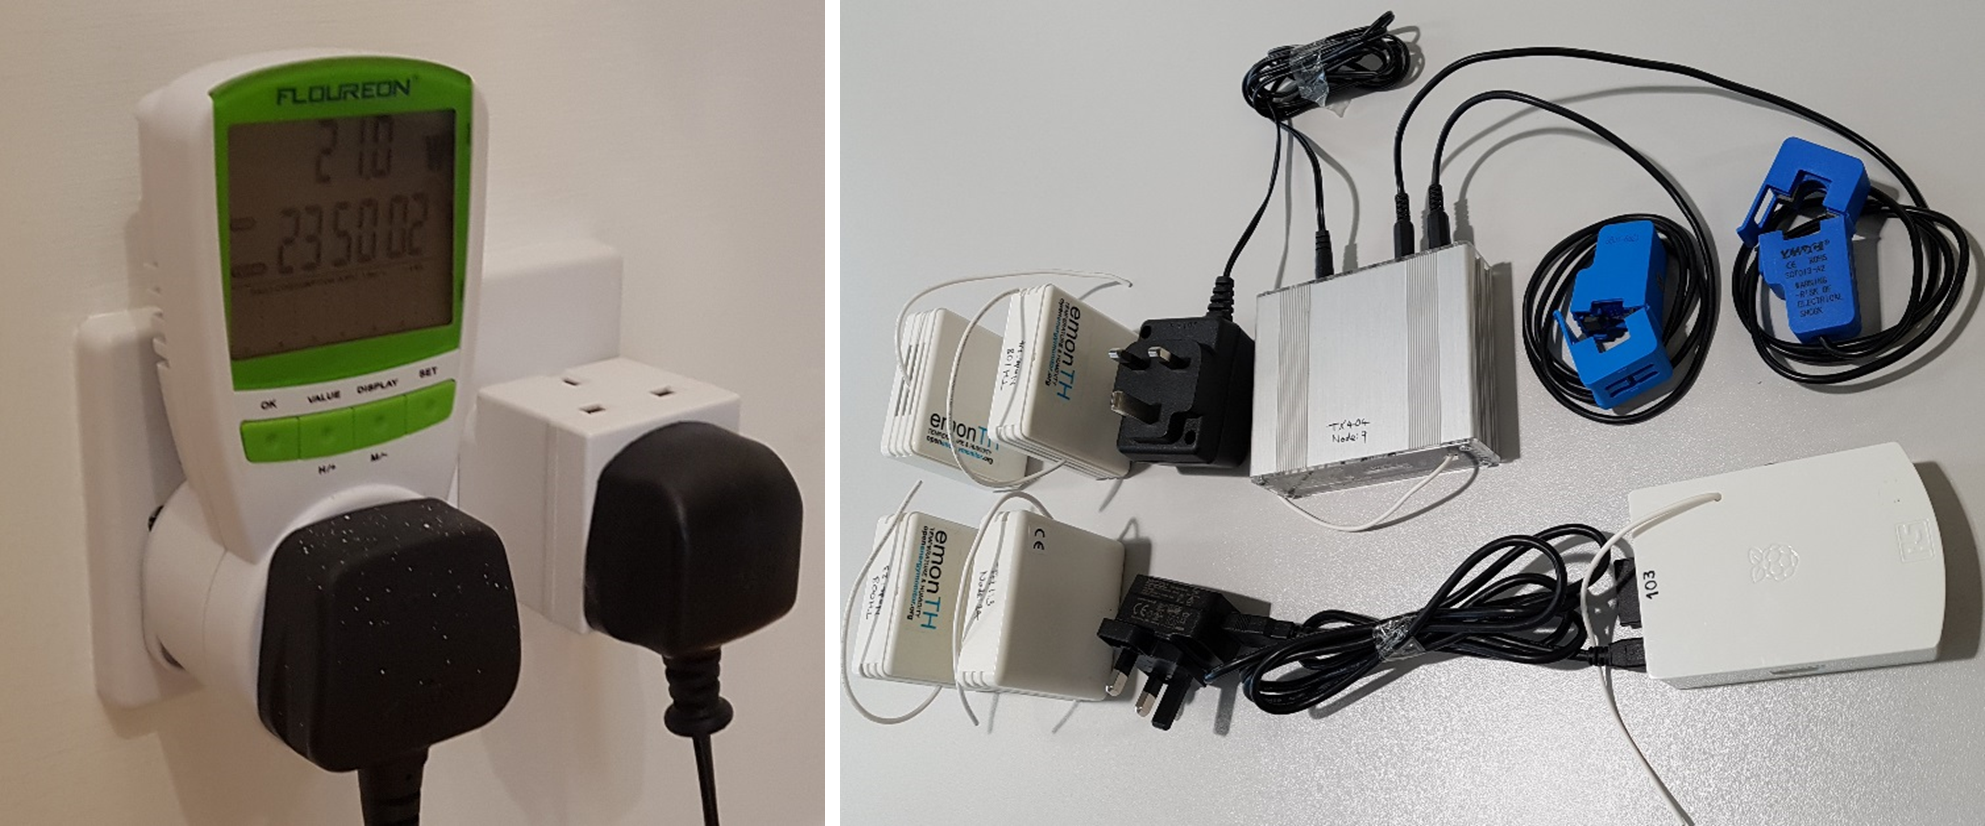
\includegraphics[width=\textwidth]{Pictures/Building/Picture1}
\caption{Left panel: power monitor used to characterise household appliances. Right panel: AC current sensor, monitoring transmitters and temperature sensors deployed in the case-study building.}
\label{Fig_Pic1}
\end{figure}

Gas consumption data was manually recorded at monthly basis using mains gas meter. Electricity consumption was logged at 10s intervals using two mains-powered clip-on current sensors on the incoming live cable providing two identical readings. The average of the two (in the end identical) readings formed the measured power usage. Gas and electricity data required no imputation.

In order to parameterise the energy model more accurately, a plugin power monitor was also used to characterise instantaneous and time-averaged consumption of the main electrical devices (TV, washing machine, ICT).

%%%%%%%%%%%%%%%%%%%%%%%%%%%%%%%%%%

\subsection{Model Input, Output and Range}\label{Subsec_InputsOutputs}

By consulting manufacturers specification and the house builder’s literature, a detailed set of parameter inputs for the model were compiled. Lower and upper bands were derived from scientific literature and used to dictate the size of associated variations explored in batch-runs (Table~\ref{Table_ranges}).  Variations in internal and external air velocities are less pronounced in ground floors, but more significant for walls and roofs. Therefore, smaller floor uncertainty margin are reported in literature (Tables~\ref{Table_ranges} and \ref{Table_all_params}: \red{Mohammad pls check correct referencing}). 

\begin{table}
\centering
\renewcommand{\arraystretch}{2}
\setlength{\tabcolsep}{4pt}
\caption{Input parameter variations explored in the batch runs used to train our Bayesian emulators. \red{Mohammad, many of these values need a careful checking between the two of us, see email :)}}
\label{Table_ranges}
\vspace{3ex}
 \begin{adjustwidth}{-2.3cm}{}
\begin{tabular}{*9c}
\toprule
 & \textbf{\small\makecell{\bf Heating \\Setpoint\\ ($^\circ$C)}} &
\textbf{\small\makecell{\bf Boiler\\Seasonal\\Efficiency\\(\%)}} &
\textbf{\small\makecell{\bf Ext.~wall\\U-value\\\red{(Unit)}}} &
\textbf{\small\makecell{\bf Roof\\U-val\\\red{(Unit)}}} &
\textbf{\small\makecell{\bf Floor\\U-val\\\red{(Unit)}}} &
\textbf{\small\makecell{\bf Infiltration\\rate (ach)}} &
\textbf{\small\makecell{\bf DHW\\Consumpt.\\(l/pers/day)}} &
\textbf{\small\makecell{\bf Cooking\\(\%)}} \\
\midrule
Short name & V1 & V2 & V3 & V4 & V5 & V6 & V7 & V8 \\
\makecell{Base-model\\Value} & $17.5$  & 65 
&  {\scriptsize\makecell{0.544 \\\red{(out of range)}}} 
&  0.213 & {\scriptsize\makecell{0.337 \\\red{(out of range)}}} 
&   0.20  & \makecell{\footnotesize \red{ to be}\\ 
                                         \footnotesize \red{discussed}} & \red{missing}
\\ 
Range &  \footnotesize $[17.5, 20.5]$   &  \footnotesize $[60, 75]$             &  \footnotesize $[0.04, 0.063]$ 
             &  \footnotesize $[0.15, 0.21]$   &  \footnotesize $[0.045, 0.055]$ &  \footnotesize $[0.2, 0.95]$ 
             &  \makecell{\footnotesize$ [6.15\times10^{-6},$\\ \footnotesize $2.2\times10^{-5}]$} 
             & $[1.05, 6.3]$\\
\bottomrule
\end{tabular}
\end{adjustwidth}
\end{table}



\begin{table}
\centering
\renewcommand{\arraystretch}{1.4}
\caption{Parameter inputs for energy model development of the case-study building. \textcolor{red}{(Dario-Mohammad: discuss caption and other red points in zoom call)}}
\label{Table_all_params}
\begin{tabular}{ll}
\toprule
{\bf Parameter} & {\bf Description} \\
\midrule
Heating                                                  & \makecell[l]{Natural gas boiler serving a radiator\\
                                                                                              central heating system} \\
Heating setpoint (setback)               &19$^\circ$C ($16^\circ$C)\\
Heating schedule                                & 02--11, 16--24\\
Ventilation                                            & \makecell[l]{Natural ventilation (mechanical extract \\
                                                                                              to family bathroom and en suite)}\\
Ventilation rate                                   & \makecell[l]{Highly stochastic, controlled by \\
                                                                                             via openable windows}\\
\red{Gas boiler  
seasonal efficiency}                           & \makecell[l]{65\% (15 year old non-condensing gas-fired \\
                                                                                             system boiler -- $77^\circ$C/$55\circ$C F+R)}\\
\red{DHW consumption}                 & $0.59$ litre/m$^2$/day \\
Cooling setpoint (setback)               & Uncontrolled \\
Nominal lighting power density     & \makecell[l]{1.4 W/m$^2$ (manually controlled) \\
                                                                                              to achieve 200 lux} \\
Number of occupants                        & 2 in total\\
Internal gains\footnote{Electricity (ICT and appliances): 3W/m$^2$; 
gas (catering): 3.3 W/m$^2$.}        & 6 W/m$^2$  \\
Gross (conditioned) area                  & $168.66$m$^2$ ($148.93$m$^2$)\\
\makecell[l]{Observed annua gas (electricity)\\ 
     consumption (2016)}                   & $15,381$ kWh ($2,991$ kWh) \\[1ex]
%{\bf \underline{Fabric properties}:} \\
%Glazing (with low emissivity coating) \\
%Glazing G Value (solar transmittance) \\
\makecell{\footnotesize\red{There were more, but are}\\
                     \footnotesize\red{already present in Table~\ref{Table_ranges}}}\\
\bottomrule
\end{tabular}
\end{table}

Manufacture’s literature for glazing (installed in 2009) stated respective G and U-values of 0.69 and 1.79 W/m$^2$K. Respective error bands of $\pm5\%$ and $\pm2\%$ for G and U- values altered the gas consumption by $\pm2.05$ kWh ($\pm 0.013\%$). Given its negligible nature, the error bands of the glazing were discounted in batch simulations. Given opaque fabric U-value impact on energy consumption \cite{kragh2017}, uncertainty bands are derived from literature and imposed on opaque U-values (Table~\ref{Table_all_params}).

Estimation of actual building infiltration rates requires convoluted air permeability tests. Table 4.16 of CIBSE guide A [6] \red{(For ref 6 see one of above notes)} outlines a range of $0.25$ to $0.95$ air change per hour (ACH) for various 2-story buildings below 500m$^2$ with a value of 0.5 ACH describing typical constructions similar to the case-study building. Therefore 0.5 ACH with a range of 0.25-0.95 ACH are used \red{(meaning of 0.5? discuss with Mohammad)}. Local weather files compiled by a weather station approximately 3 miles away from the site was used to support the model development \red{[27] (M: can you pls provide bibtex version of old reference 27)}. 

We therefore consider eight uncertain parameters (Table~\ref{Table_ranges}), and use monthly gas and electricity consumption and hourly temperature data to history-match them.  In the following, we will use the parameter to refer to any of the eight uncertain quantities in Table~\ref{Table_ranges}, and the term input to refer to a specific configuration of the eight parameters $\x = (x_1, \dots, x_8)$.


%%%%%%%%%%%%%%%%%%%%%%%%%%%%%%%%%%
%%%%%%%%%%%%%%%%%%%%%%%%%%%%%%%%%%
%%%%%%%%%%%%%%%%%%%%%%%%%%%%%%%%%$

\section{Results}
\label{Sec_Results}
This section discusses the results of the application of the statistical principles and methods of Section~\ref{Sec_Methods}, to the example study of Section~\ref{Sec_Example}. We build emulators of the model outputs of interest and history-match these outputs to identify a region of non-implausible inputs. 

%%%%%%%%%%%%%%%%%%%%%%%%%%%%%%%%%%

\subsection{Experimental Design and Simulated Results}

To build emulators of the model outputs, results of a small number of model runs are needed. An informal rule of thumb suggests using about 10 times as many runs as the number of varied parameters (eight in our case) \cite{loeppky2009}. In our case the simulator was moderately fast to evaluate, and a total of $n=1,000$ simulations were run (taking about 16 hrs in E+). Note that this is substantially more than what is typically needed for eight inputs. While the results presented here are obtained by exploiting the information from all 1,000 runs, we have also simulated a more typical case where only 100 runs (randomly selected among the original 1,000) were used. This however yields no difference to the final results (see Section~\ref{Sec_Discussion}). 

The experimental design (the set of $n$ inputs for which the simulator is run) was chosen through Latin Hypercube Sampling (LHS). In two dimensions, the technique selects n points in a square so that exactly one point falls in each row and in each column of an $n\times n$ uniform grid of the square.  The same idea governs higher dimensions. For this reason, LHS is commonly used in the design of computer experiment analyses \cite{vernon2010galaxy, lord2017, pope2021}, to identify points in a hypercube that fill the space well and are not too close to each other \cite{mckay2000}. LHS is easily performed in R via the “lhs” package.


\subsubsection{Gas}

Fig.~\ref{Fig_gas_histograms} shows simulated and observed values of monthly gas consumption for the $1,000$ design runs. A distinction between summer and non-summer months can be noticed: in June, July and August, all model runs considerably underestimate the observed consumption. This, in principle, does not rule out the possibility that other inputs within the explored space (an eight-dimensional hypercube with side ranges as in Table~\ref{Table_ranges}) may lead to a match. In this case, however, especially in June and July, it is evident that the range of simulated outputs is small with respect to the distance between these and the observed consumption: a simple linear model confirms indeed that a match within the explored space cannot be achieved for these months.

\begin{figure}
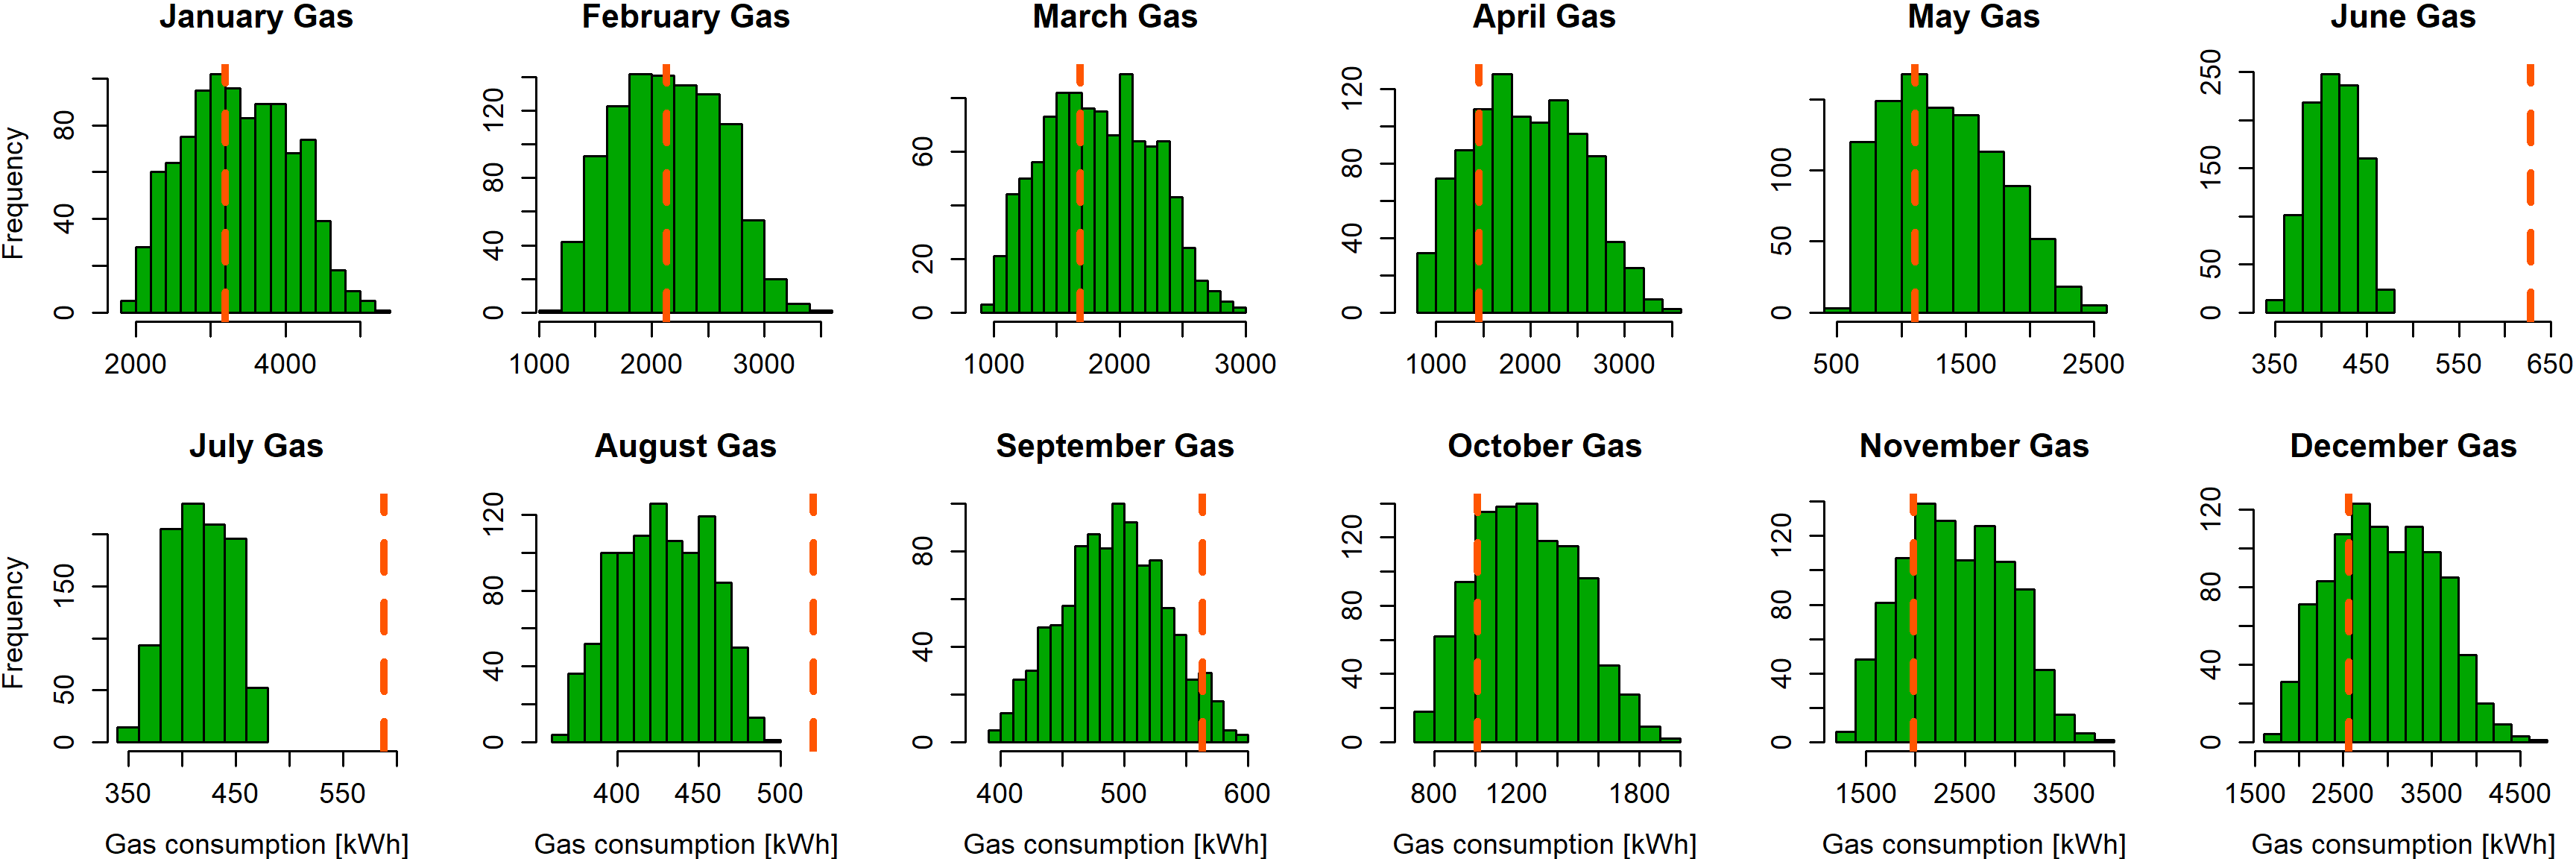
\includegraphics[width=\textwidth]{Simulation_histograms/Batch_2_only/Gas_Runs/All_months_gas_2x6}
\caption{Distribution of simulated monthly gas consumption, for the experimental design used in this study ($n=1000$ inputs). The dashed vertical line in a plot denotes the observed consumption for that month. Note that, for Jun-Jul-Aug, this lies outside of (and often far from) the range of simulated consumptions.}
\label{Fig_gas_histograms}
\end{figure}

As illustration of the proposed methodology, in the following we will look for inputs that match all nine non-summer monthly gas consumption simultaneously, excluding the three summer conditions from the match. It is important to note that in a real case study, the model’s underestimation of summer consumptions should be identified and acted upon, prior to calibration/history matching. While the most likely reason for summer months deviation is the inability of deterministic schedules to capture stochastic aspects of energy governance in the household (\textit{i.e.}, additional use of hot water/cooking in these months), our intervention with the model to reflect historical occupant behaviour for which we had little certainty would have been speculative. Greater insight into seasonal energy use variations would have allowed one or more parameters to be added as additional input variables to be history-matched. 


\subsubsection{Electricity}

As described in Section~\ref{Subsec_InputsOutputs}, the model also predicts monthly electricity consumption. Within the explored ranges of the parameters, however, all months display almost no variability in output, with an observed consumption far outside the range of simulated values. For the three summer months (Jun--Aug), no variation at all is shown in simulated consumption among the $n$ runs. This is partly an outcome of the deterministic electrical load specification. More importantly though, this is due to the fact that any changes with the 6 variables in Table~\ref{Table_ranges} except for heating and DHW (V1 and V7) will only affect gas consumption. This makes the variability of electricity consumption very limited and bound to a small deterministic input schedule (e.g., a fixed 6 W/m$2^2$ for internal gains as dictated by field measurements). 

Given the illustrative role of the example study within this work, we will not attempt to match the electricity consumptions in the methodological illustration that follows. We will instead consider the nine conditions coming from the observed monthly gas consumption in non-summer months, to which we will add temperature constraints in Section~\ref{Subsec_Temperature}. 

%%%%%%%%%%%%%%%%%%%%%%%%%%%%%%%%%%

\subsection{Emulation of Monthly Gas Consumption}

For each of the nine non-summer months, the $n=1,000$ simulations provide a dataset of n pairs $(\x[i], y_i)$ where $\x[i]$ represents one configuration of the 8 input parameters, and $y_i$ is the simulated gas consumption associated with it. We use the dataset to build an emulator of that month’s gas consumption. To that aim, the eight input parameters are linearly rescaled so that each of them ranges in the interval $[-1,1]$.
 
From Section~\ref{Subsec_Emulators}, recall that several choices (on covariates, correlation lengths, prior variances) have to be made when building an emulator. To validate these choices, we split the dataset as follows:
\begin{itemize}
\item Training set (700 runs): used to train the emulators.
\item Evaluation set (150 runs): used to decide on the values of the emulator hyperparameters, by comparing the emulator's performance on this set to the known simulator's outputs.
\item Test set (150 runs): used to test the previously built emulators on a completely new set of runs not used for training and evaluation.
\end{itemize}
Following the notation of Section 3.1, the prediction of the simulated consumption at an input  $\x$ is computed as sum of: i) a linear regression part, ii) a prediction of the regression residual at the point $\x$, in the form of a Bayes linear emulator. Details on each of the two parts follow.

%%%%%%%%%%%%%%%%%%%%%%%%%%%%%%%%%%

\subsubsection{Linear Regression}\label{Subsec_LR}

The only choice to be made in building a linear regression model concerns the predictors to use, \textit{i.e.}, the functions $g_i$ in equation~\eqref{eqn_emulator}. For all the months of interest, a preliminary exploration reveals that the response $y$ (gas consumption) is very well explained as quadratic function of the eight input parameters, which in the following we call  $V_1, \dots, V_8$ for convenience. Thus, we proceed as follows.

Let $\mathcal{P}$ be the set of all mutually orthogonal linear, quadratic and interaction terms of $V_1, \dots, V_8$.\footnote{Obtained in \texttt{R} via the command \texttt{poly(X, deg=2)}, where \texttt{X} is the $700 \times 8$ matrix whose rows are the training inputs. For 8 parameters, there is a total 44 linear, quadratic and interaction terms.}
For a given integer $k$, consider the linear model with highest adjusted coefficient of determination (adj.~$R^2$) and consider the smallest integer $k$ for which the above linear model with $k$ predictors has an adj.~$R^2$ exceeding the threshold.

In our case, 10 predictors yield models with notably high adj.~$R^2$, about $0.999$ across all months. To keep the approach uniform among months, we consider the linear model with the “best” 10 predictors for each month (Table~\ref{Table_Emulator}). As pointed out above, however, a different number of predictors for each output may be considered on other case studies. 

\begin{table}
\centering
\renewcommand{\arraystretch}{2}
\setlength{\tabcolsep}{1.5ex}
\caption{Properties of the gas consumption emulators. For each month, from left to right: covariates used to build the linear regression model; adjusted $R^2$ of the linear model; variance of the residuals; active parameters used in the covariance function; value of the correlation lengths (same for all active parameters). In the predictor’s column, the * symbol denotes the combination of all linear and interaction terms: $a*b*c$ = \{$a, b, c, ab, ac, bc$\}.
}
\label{Table_Emulator}

\begin{tabular}{*6c}
\toprule
                   &  {\bf Predictors}  &   {\bf Adj.~$\bd{R^2}$}  &   $\bd{\sigma^2}$  &   {\bf Act.~Params}  & $\bd d$  \\
\midrule
 {\bf Jan}   & $V_1*V_2*V_6, V_3, V_4, V_2^2, V_6^2$  & 0.9998  &  85.94  & $V_1, V_2, V_3, V_6, V_8$ & 0.8 \\
 {\bf Feb}   & $V_1*V_2*V_6, V_3, V_4, V_2^2, V_6^2$  & 0.9997  &  52.30  & $V_1, V_2, V_3, V_7, V_8$ & 0.65 \\
 {\bf Mar} &  $V_1*V_2*V_6, V_3, V_4, V_2^2, V_6^2$ & 0.9997  &  50.14  & $V_1, V_2, V_3, V_6, V_7, V_8$ & 1.3 \\
 {\bf Apr}  & $V_1*V_2*V_6, V_3, V_4, V_2^2, V_6^2$ &  0.9998  &  50.04  & $V_1, V_2, V_3, V_6, V_8$ & 1 \\
 {\bf May} & $V_1*V_2*V_6, V_3, V_8, V_1^2, V_6^2$ &  0.9989  & 206.45 & $V_1, V_2, V_3, V_4, V_6, V_8$ & 1 \\
 {\bf Sep}  & $V_1*V_2*V_6, V_3, V_4, V_8, V_6^2$      &  0.9994  &   0.91    & $V_1, V_2, V_3, V_6, V_7, V_8$ & 1.2 \\
 {\bf Oct}  &  $V_1*V_2*V_6, V_3, V_4, V_8, V_6^2$     &  0.9996   &  24.40  & $V_1, V_2, V_3, V_6, V_7, V_8$ & 1.4 \\
 {\bf Nov} & $V_1*V_2*V_6, V_3, V_4, V_2^2, V_6^2$ &  0.9998  &  57.35   & $V_1, V_2, V_3, V_6, V_7, V_8$ & 1.2 \\
 {\bf Dec} & $V_1*V_2*V_6, V_3, V_4, V_2^2, V_6^2$  &  0.9998  &  68.77  & $V_1, V_2, V_3, V_6, V_7, V_8$ & 1.3 \\
 \bottomrule
\end{tabular}
\end{table}

Note that, in general, such a high $R^2$ should raise concerns of overfitting. In our case, the concern can be ruled out by observing that only 10 predictors have been used to explain 700 observations. The high coefficient of determination mirrors an intrinsically quadratic model dynamics.

%%%%%%%%%%%%%%%%%%%%%%%%%%%%%%%%%%

\subsubsection{Emulators of the Residuals}

To build an emulator of the regression residuals of each month’s consumption, choices about the following quantities are to be made: active parameters $\x[A]$, correlation lengths $d_i$, prior emulator variance $\sigma_u^2$ an nugget variance $\nu^2$ - see equation~\eqref{eqn_kernel} and text thereafter. We proceed as follows.
\begin{itemize}
\item {\bf Active parameters $\x[A]$}: To identify them, we look at the most significant (in the sense discussed in Section~\ref{Subsec_LR}) second- and third- order terms in a linear regression model of the residuals. Variables appearing by themselves with a high $t$-value ($t>8$) are included as active parameters. The inclusion of variables appearing alone with a lower t-value or in interaction with other variables is instead considered case by case, according to the emulator performance on the evaluation set – see Section~\ref{Subsec_Validation}.
\item {\bf Correlation lengths $d_i$}: Once the active parameters are chosen, the same correlation length $d$ is used for all of them. The value of $d$ at each month is chosen by assessing the emulator's performance on the evaluation set and is reported in Table~\ref{Table_Emulator}. Notice that, to attain a similar level of correlation across the space, higher correlation lengths are used when a higher number of active parameters is present.
\item {\bf Prior variances $\sigma_u^2$ and $\nu^2$}: Let $ \sigma^2$ denote the variance of the regression residuals being fitted. Hence, we set $\sigma_u^2 = 0.95 \sigma^2$ and $\nu^2 = 0.05 \sigma^2$.
\end{itemize}

Table~\ref{Table_Emulator} provides details of all choices made to build each of the nine emulators, including the ones concerning the regression line. We discuss validation of the emulators in the next section.

%%%%%%%%%%%%%%%%%%%%%%%%%%%%%%%%%%

\subsubsection{Emulator Validation and Performance}\label{Subsec_Validation}

The active parameters $\x[A]$ and correlation lengths $d$ in Table~\ref{Table_Emulator} are chosen based on the emulator’s performance on the evaluation set. The latter consists of 150 pairs $(\x[i], y_i)$ not used in the emulator’s training, where each $y_i$ is the simulated output at input $\x[i]$. At each such $\x[i]$, the emulator provides a prediction $\hat y_i$ of the simulated output and an uncertainty statement about the prediction in the form of a standard deviation $\hat\sigma_i$. One way to assess the emulator’s performance at $\x[i]$ is thus to define: 
\begin{equation}\label{eqn_st_error}
\varepsilon_i = \frac{\hat y_i - y_i}{\hat \sigma_i}\,.
\end{equation}
We call $\varepsilon_i$ the emulator standardised error at $\x[i]$. It represents the number of standard deviations which separate the emulator prediction from the known simulated output.

As we make no distributional assumption on the emulator, we can appeal to Pukelsheim’s $3\sigma$ rule \cite{3sigma} to constrain expected values of $\varepsilon_i$: the result states that, for any continuous unimodal distribution, at least $95\%$ of the probability mass lies within 3 standard deviations from the mean. Therefore, by only assuming unimodality of the emulator distribution, we should expect at least $95\%$ of the $\varepsilon_i$ to lie between -3 and 3. 

For each of the nine emulators, we consider the plot of $\varepsilon_i$ versus the predictions $\hat y_i$. Given a good emulator, such a plot should be characterised by an approximately random scattering of the points around the line $\varepsilon=0$, with about $95\%$ of them in modulus less than 3 due to Pukelsheim’s rule. We assess visually both these properties for different choices of active parameters and correlation lengths, choosing the ones which return plots with the desired properties. 

We tend to be slightly conservative in this phase, by choosing correlation lengths which generally yield more than $95\%$ of $|\varepsilon_i|$ less than 3 . This is to prevent making choices tailored to the specific points used for validation. Once the parameters $\x[A]$ and $d$ are chosen, we compute the standardised errors in equation~\eqref{eqn_st_error} on the 150 elements of the test set, to check that no anomaly shows up on a set of points never used in training or evaluation.

Finally, we note that the emulators of the nine monthly gas consumptions are remarkably precise in their predictions. This is a consequence of both an excellent regression fit to the data, and of a further reduction in the residual uncertainty due to the emulators. Quantification of this reduction is provided in Table~\ref{Table_variance}, which shows the original variance of the residuals and an empirical $95\%$ confidence interval (CI) of the emulator variance on the 150 test points. The CIs show that the uncertainty in the emulator predictions is very small compared to the range of simulated outputs (Fig.~\ref{Fig_comparison_LR}). 


\begin{table}
\centering
\renewcommand{\arraystretch}{2}
\setlength{\tabcolsep}{1.5ex}
\caption{For each month: variance of the regression residuals to which the emulator is fitted (first row); empirical $95\%$ confidence interval of the emulator variance on the 150 test points (second and third row).}
\label{Table_variance}
\begin{tabular}{*{10}c}
\toprule
                   & \bf Jan & \bf Feb & \bf Mar & \bf Apr & \bf May & \bf Sep & \bf Oct & \bf Nov & \bf Dec \\
\midrule
$\bd \sigma^2$   & 85.9 & 52.3 & 50.1 & 50.0 & 206.4 & 0.91 & 24.4 & 57.4 & 68.8 \\
$\bd{[2.5\%,}$    &  6.6  &  5.9  &   3.1  &  3.2  &  16.8   & 0.06 &  1.5  &   3.8  &  4.3  \\
$\bd{[97.5\%]}$ & 31.0 & 28.0&   9.3  & 10.0 &  68.9   & 0.20 &  3.8  & 12.8 & 12.7 \\
 \bottomrule
\end{tabular}
\end{table}


\begin{figure}
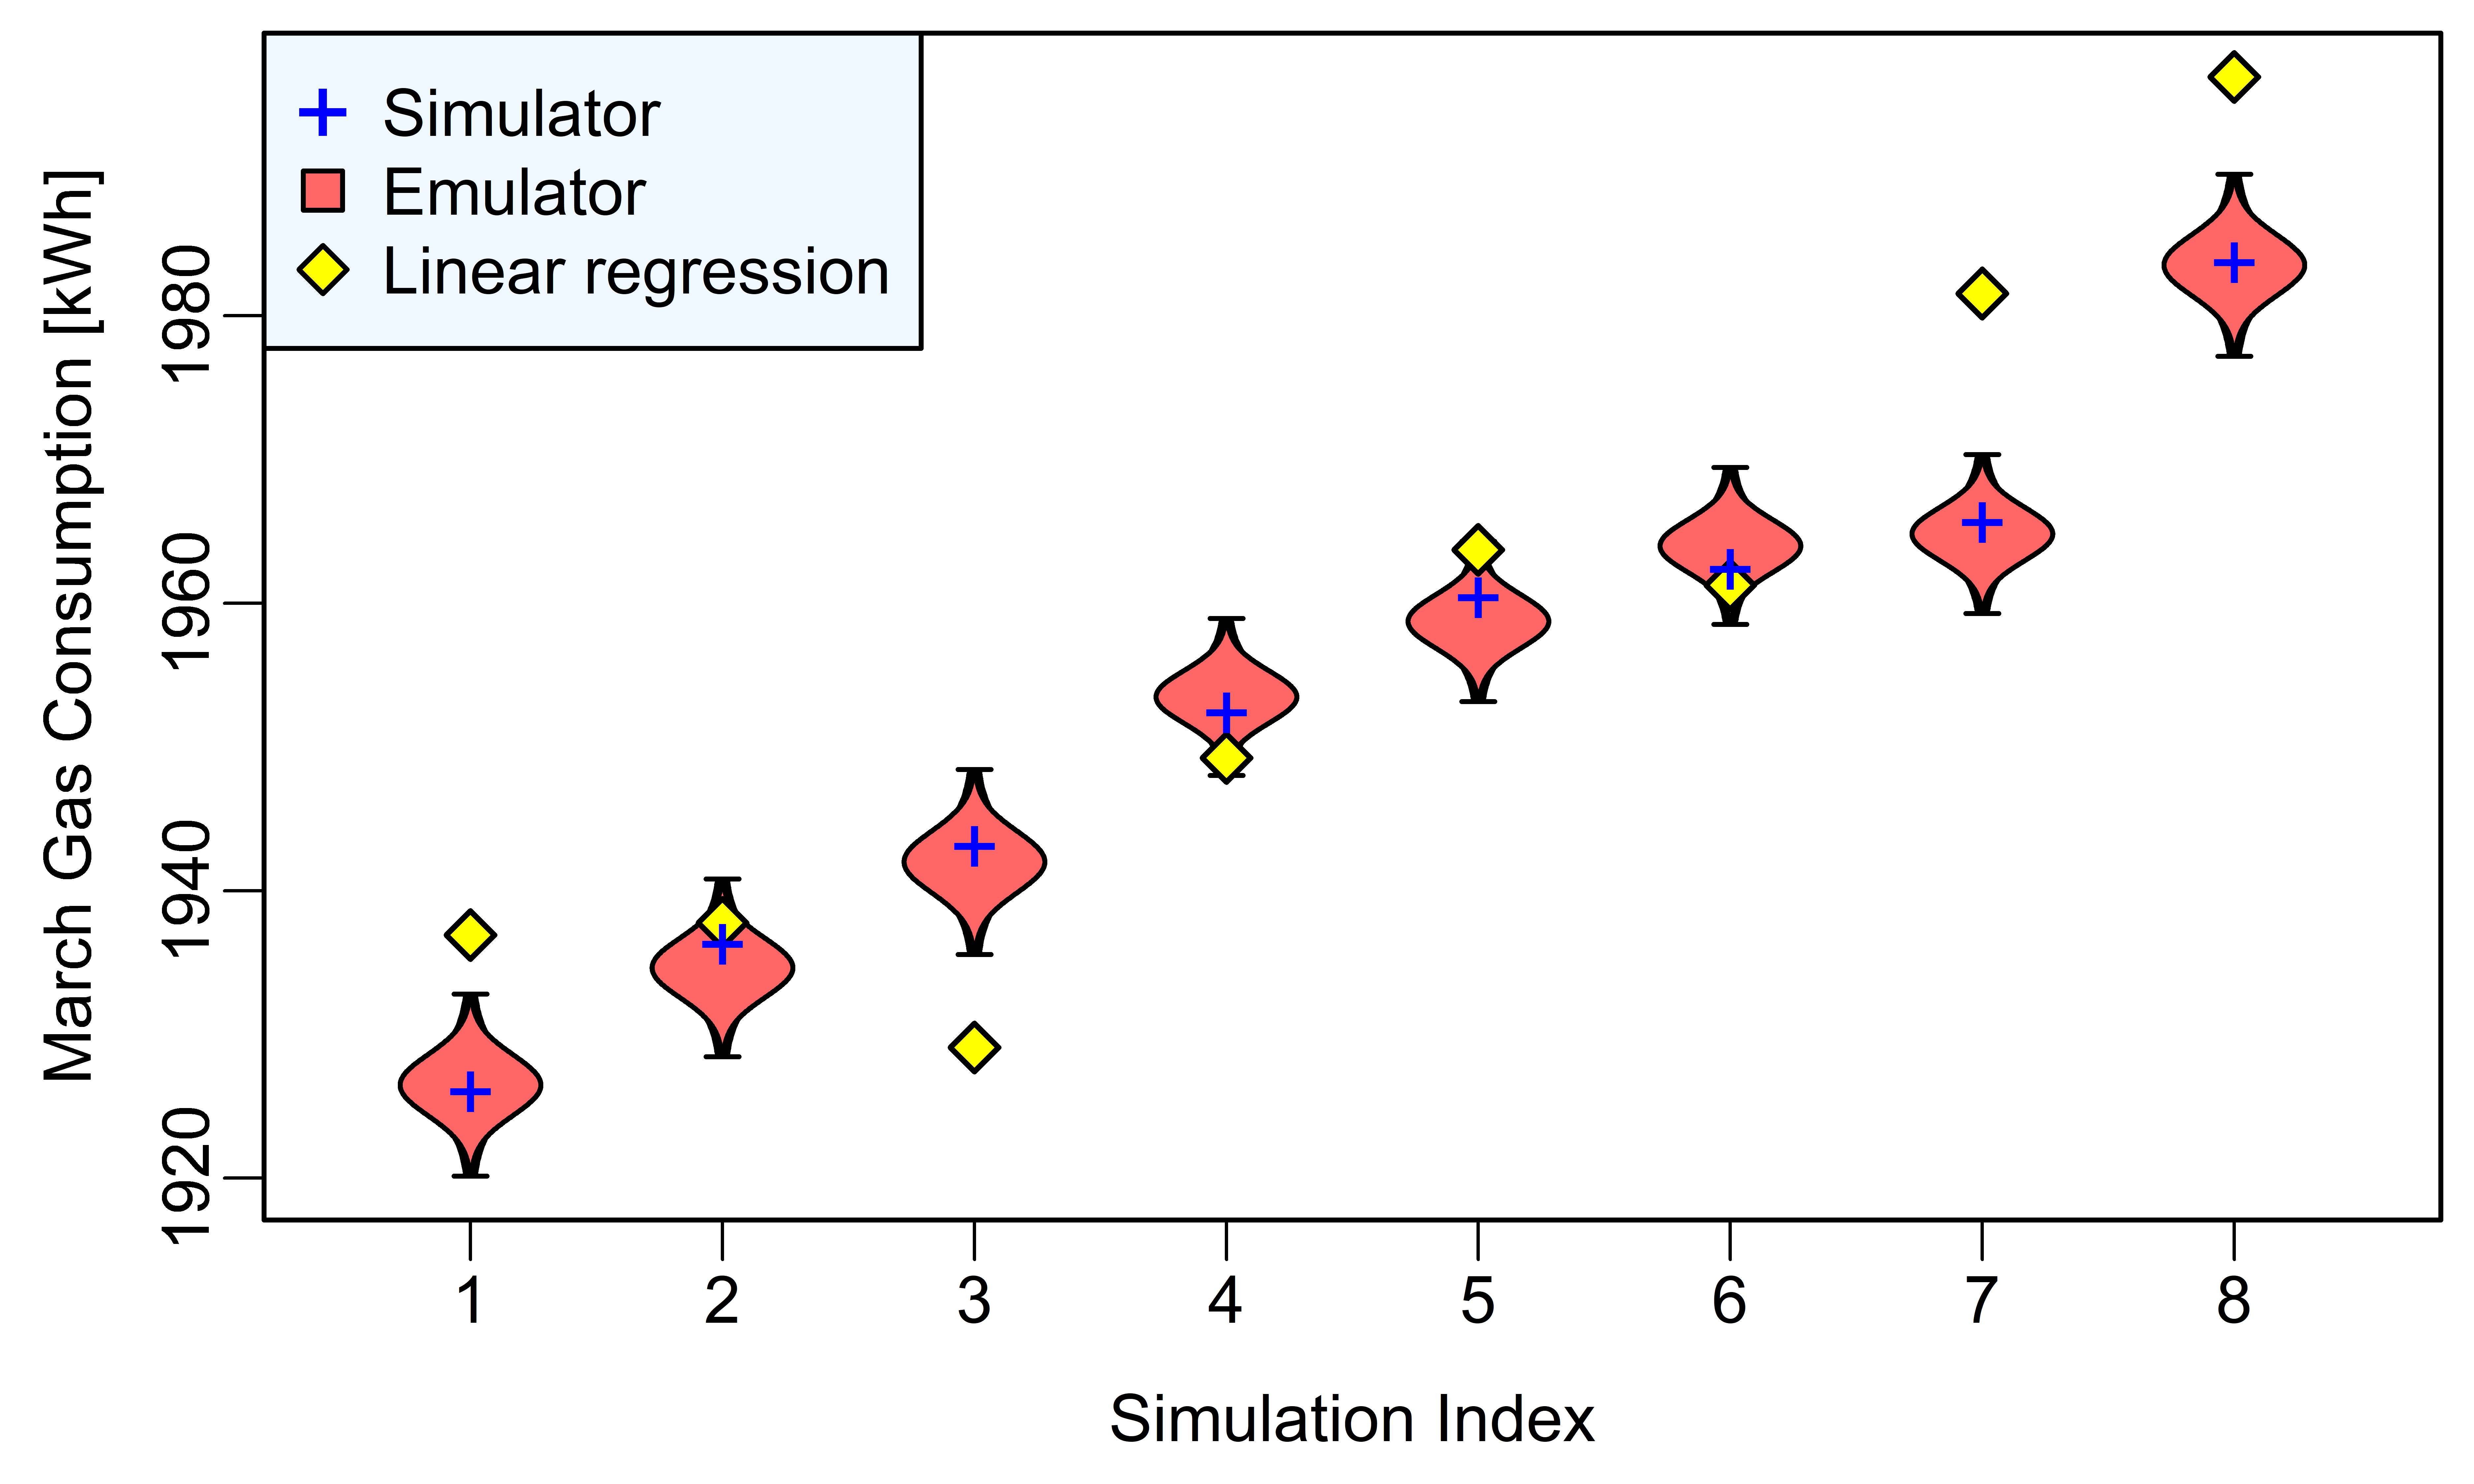
\includegraphics[width=\textwidth]{Validation_Plots/Comparison_LR/LR_Mar_82-89.png}
\caption{Comparison between point regression predictions and emulator predictions with associated uncertainty, for a sequence of randomly selected eight consecutive simulated March gas consumptions of the test set. The bell-shaped curves cover a range of 3 emulator standard deviations up and down the emulator prediction; the simulated value (+) always lies within this range, while the regression prediction may lie substantially further. Results are displayed for eight simulations to have a small  range in the $y$-axis and allow to appreciate detail. }
\label{Fig_comparison_LR}
\end{figure}

%%%%%%%%%%%%%%%%%%%%%%%%%%%%%%%%%

\subsection{Observational Error and Model Discrepancy}\label{Subsec_OEandMD}

The validated emulators can be used as probabilistic surrogate of the original model, to predict the monthly gas consumption at any input $\x$. We use the implausibility measure described in Section~\ref{Subsec_IM} to compare the prediction with the observed consumption $z$. The observational error ($e_{OE}$) and model discrepancy ($\varepsilon_{MD}$) are set as follows:
\begin{enumerate}
\item The OE is set to $5\%$ of the observed value $z$, in agreement with the largest manufacturer’s accuracy band ($\pm 5\%$ for power monitor).
\item 	For illustrative purposes, we set MD to either $10\%$ or $20\%$ of the emulated consumption and compare results in the two cases.
\end{enumerate}
Note that, as discussed in Section~\ref{Subsec_MD_Energy}, accurate estimation of model discrepancy requires careful statistical analysis and possibly additional model runs. However, an order of magnitude between $10$ and $20$\% of the simulated values is likely to represent a good estimate in many energy applications. If there are reasons to believe that model discrepancy is much higher, then the possibility of revisiting the model itself should be considered, by possibly including in the model key factors affecting the simulated dynamics.

%%%%%%%%%%%%%%%%%%%%%%%%%%%%%%%%%%

\subsection{History Matching}

The HM procedure has been described in Section~\ref{Subsec_HM}. In our case, at an input configuration $\x$:
\begin{enumerate}
\item We first compute the implausibility measures $I_M (\x)$ for months M, as in equation~\eqref{eqn_IM};
\item We then define the overall implausibility $I(\x)$ as in equation~\eqref{eqn_IM_overall}, $I(\x) = \max_M I_M(\x)$;
\item Hence, we consider an input as non-implausible if $I(\x) < 4$.
\end{enumerate}

As explained in Section~\ref{Subsec_HM_comments}, choosing a higher threshold than the more common $T=3$ ensures that the probability of incorrectly rejecting an input $\x$ as implausible is kept small, whenever several observations are being matched simultaneously (nine in our case). Also notice that an alternative approach may be to define $I(\x)$ as the second- or third-highest value of $I_M (\x)$ over all months, while keeping a relatively low threshold $T$. However, if a particular month proves more challenging to match, this approach risks to classify several points as non-implausible, although those points are highly unlikely to match the observed consumption for that month.

In our example study, the percentage of space classified as non-implausible after one wave is $0.30\%$ when $10\%$ MD is used, and $19.52\%$ for $20\%$ MD. These percentages have been estimated by computing the proportion of non-implausible points on a sample of size $N=10^7$, generated via a Sobol sequence in the eight-dimensional unit hypercube. The relative error on these estimates (approximately equal to $\left[(p(1-p)/N\right]/p$, where $p$ is the estimated fraction) is therefore order of $10^{-2}$ and $10^{-3}$ in the two cases respectively. This makes both estimates very accurate.


In this case, we do not need to proceed to further waves. For all the months, the emulator uncertainty (Table~\ref{Table_variance}) is already 1-2 orders of magnitude lower than the combined one from MD and OE. Additional waves therefore leave the implausibility measure essentially unchanged. We comment further on this in Section~\ref{Sec_Discussion}.

%%%%%%%%%%%%%%%%%%%%%%%%%%%%%%%%%%

\subsubsection{Visualisation of the Non-Implausible Region}

The non-implausible region lives in an eight-dimensional space, one dimension per input parameter. To identify variables which play a role in constraining the region, we look at two-dimensional scatter plots of the non-implausible points, for all possible pairs of the 8 variables. For brevity, we do not show these all here. However, in the $10\%$ MD case, the plots reveal that two variables are particularly significant: infiltration rate ($V_6$) and cooking energy consumption ($V_8$). One additional variable (heating setpoint, $V_1$) also seem to play a role in identifying non-implausible points.

Fig.~\ref{Fig_NI_gas_10} contains minimum-implausibility (MI) and optical-depth (OD) plots for all pairs of the three above variables. The MI plot of a pair of parameters shows the minimum value of the implausibility measure $I(\x)$ over the hidden six dimensions. Thus, values greater than $T=4$ in a MI plot identify pairs of the two parameters in question that will always be classified as implausible, irrespectively of the value taken by the remaining six parameters. For values smaller than $T=4$, the OD plots instead show the fraction of non-implausible points, in the hypervolume extending over the six hidden dimensions. 

\begin{figure}
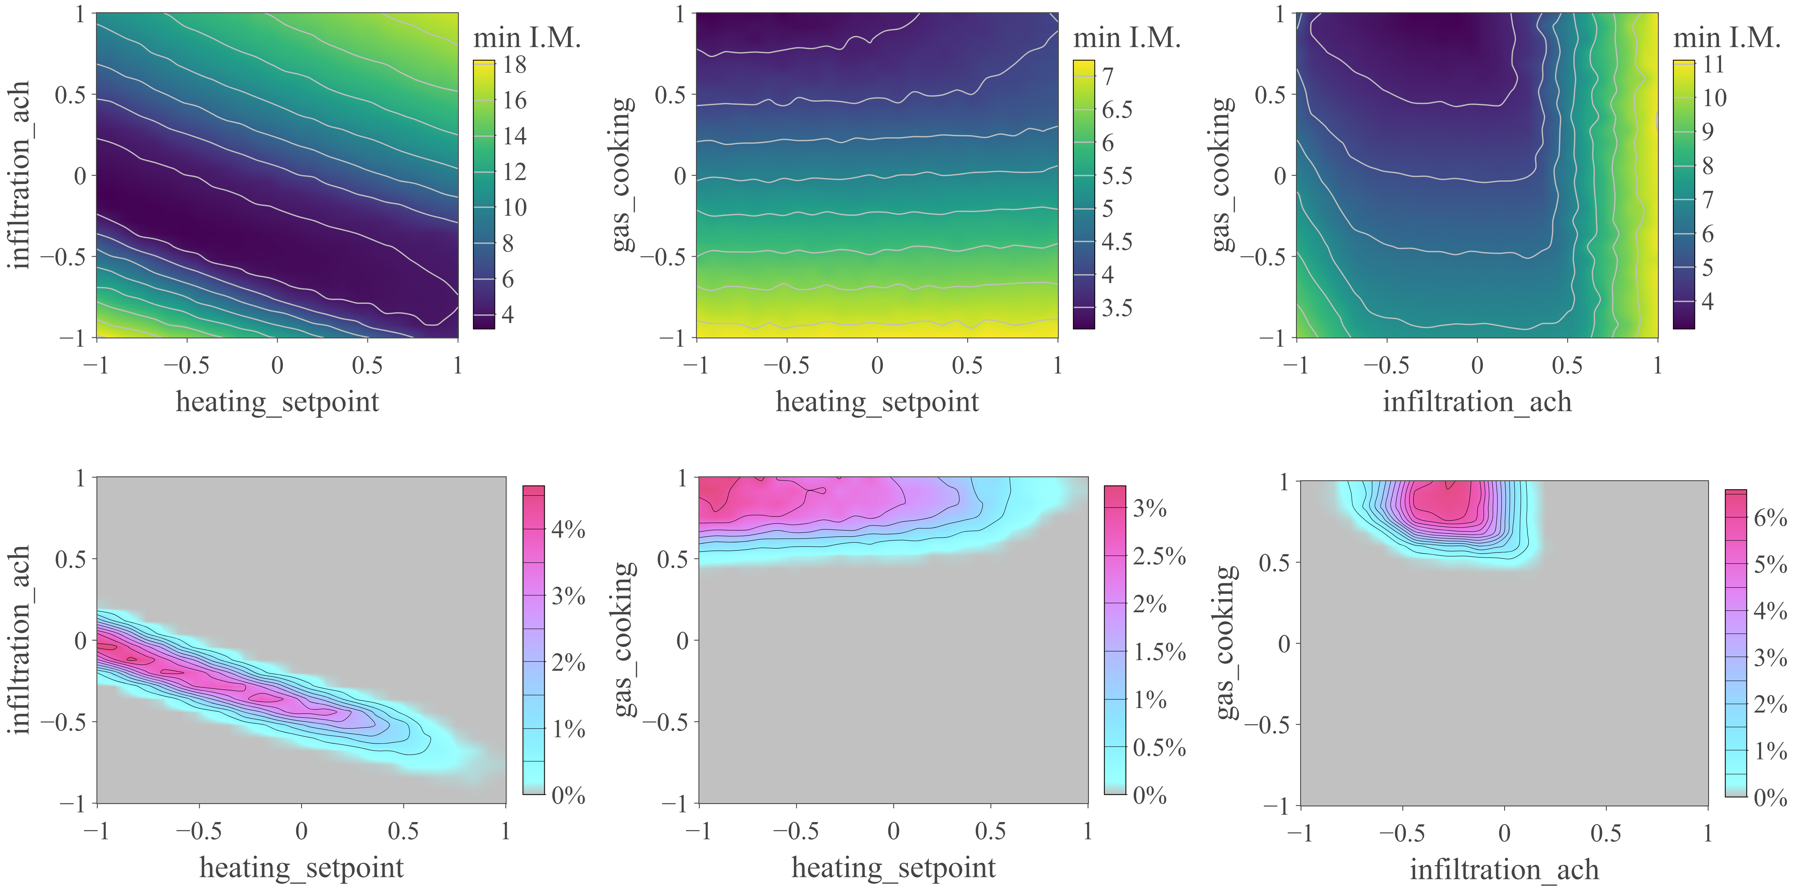
\includegraphics[width=\textwidth]{Non-Implausible_Plots/Gas/Fig1}
\caption{Plots of the non-implausible space when $10\%$ MD is considered. Each panel in the top row shows the minimum implausibility along the six dimensions not included in the plot. Panels in the bottom row show the percentage of non-implausible region along the hidden dimensions.}
\label{Fig_NI_gas_10}
\end{figure}

Fig.~\ref{Fig_NI_gas_10} reveals that only values of the gas cooking higher than $5\%$ of total household energy demand are able to yield a match with the observed monthly consumptions. Moreover, within the explored ranges, such values should be paired with values of the infiltration rate (right panels) approximately between 0.25 and 0.65 ach \red{uniformity in lower/capital ach. Mohammad, preference?)}. Note that the two variables seem to be relatively independent. A stronger dependence can be seen instead for non-implausible values of heating setpoint and infiltration rate (left panels). Heating setpoint values are by themselves only minimally contrained: however, higher infiltration rates yield more constrained, lower values of the heating setpoint. 

The left subplots in Fig.~\ref{Fig_NI_gas_10} also suggest that non-implausible values of the heating setpoint may as well be found to the left of the range originally deemed appropriate for this input variable. A similar consideration is valid for gas cooking values higher than the relevant range. Similar findings are not uncommon, especially during a first wave of HM. In such a case, it is advisable to step back and expand the ranges in question, running additonal simulations in the new region before proceeding with HM. However, for brevity purposes and in accordance with the methodological aim of the work, in this illustrative example we limit our discussion to the hypercube with ranges specified in Table~\ref{Table_ranges}.

%%%%%%%%%%%%%%%%%%%%%%%%%%%%%%%%%%

\subsubsection{Sensitivity to Model Discrepancy Magnitude}

The plots in Fig.~~\ref{Fig_NI_gas_10} concern the case where the magnitude of model discrepancy is $10\%$. Fig.~\ref{Fig_NI_gas_20}  shows MI and OD plots for the same three variables, in the case of $20\%$ MD. Roughly, similar patterns to the ones of Fig.~\ref{Fig_NI_gas_10} emerge, albeit spread over larger regions: due to a lower confidence in the model, we rule out fewer points as implausible. The percentage of non-implausible points has risen to $19.52\%$, from only $0.3\%$ in the $10\%$ MD case. 

\begin{figure}
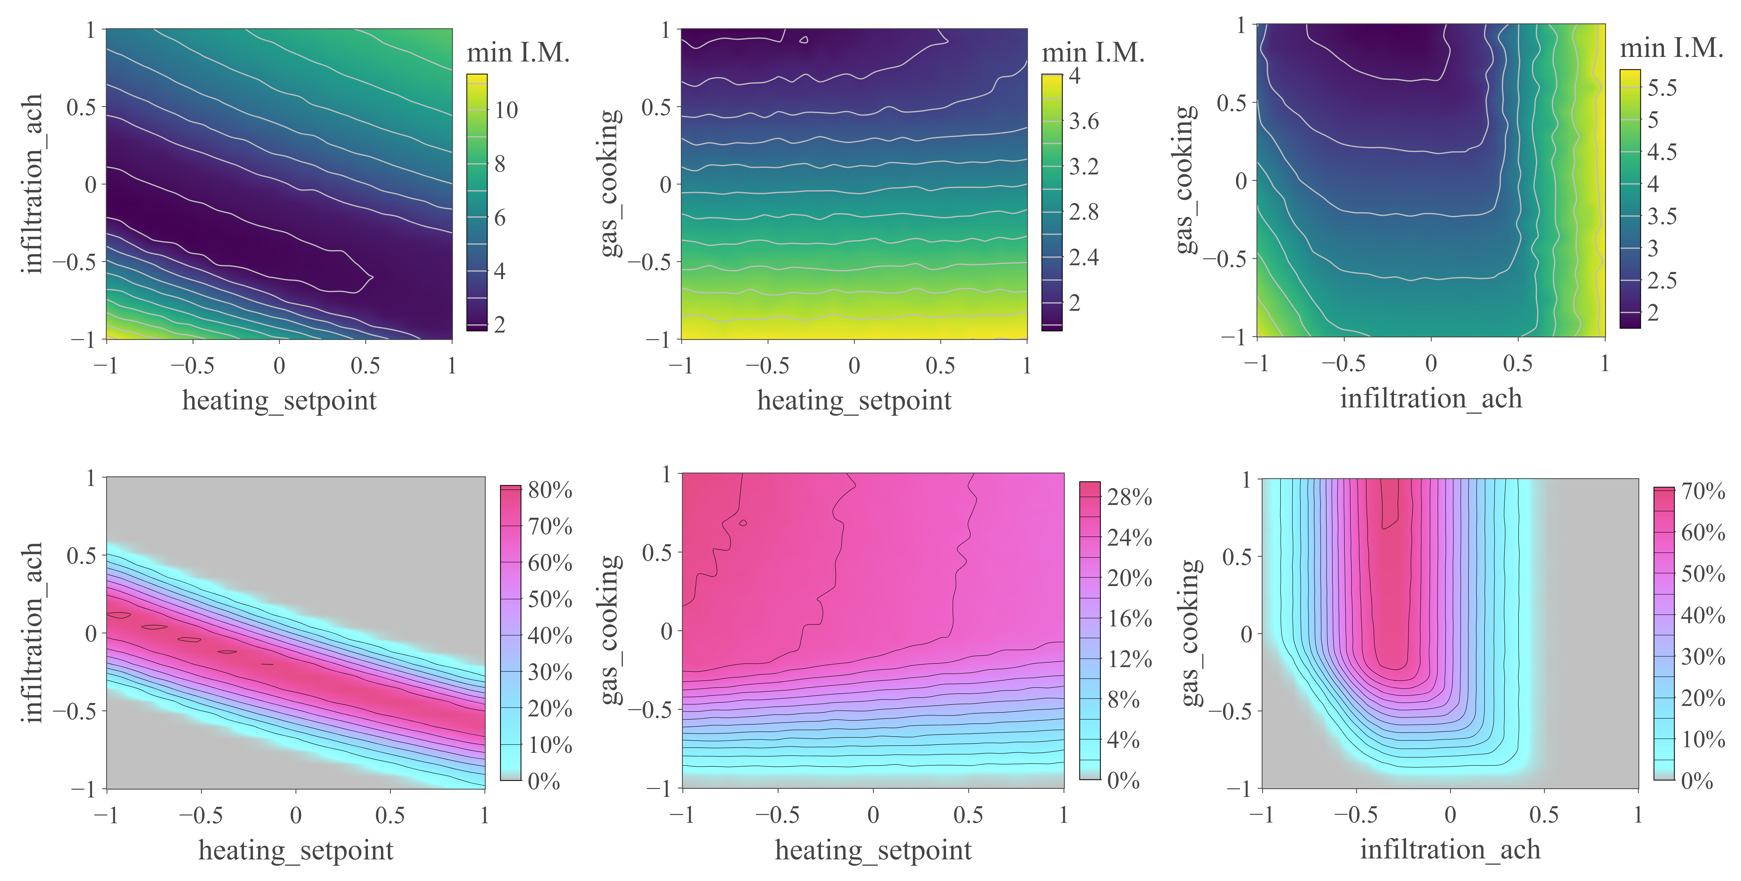
\includegraphics[width=\textwidth]{Non-Implausible_Plots/Gas/Fig2}
\caption{Same content as in Fig.4, when $20\%$ MD is considered. Each panel in the top row shows the minimum implausibility along the six dimensions not included in the plot. Panels in the bottom row show the percentage of non-implausible region along the hidden dimensions.}
\label{Fig_NI_gas_20}
\end{figure}

This comparison highlights the potential sensitivity of history matching results to the choice of MD. Note that the precision of the emulator(s) used also plays a role in this. In our case, as Table~\ref{Table_variance} shows, we have remarkably precise emulators. Hence, essentially all the uncertainty accounted for in comparing emulator predictions and observations comes from model discrepancy and, to a lower extent, measurement error. Doubling the MD will thus make points significantly more likely to be deemed non-implausible. This once more highlights the importance of assessing the right order of magnitude of model discrepancy prior to performing history matching, as discussed in Sections~\ref{Subsec_Limitations} and \ref{Subsec_MD}.

%%%%%%%%%%%%%%%%%%%%%%%%%%%%%%%%%%

\subsubsection{Role of Different Constraints and Correlation among Outputs}

The emulators allow to explore a wide range of questions, for which it would otherwise be impossible to draw sound inference. We briefly discuss one such example here, by looking at the compatibility between the imposed constraints (observed consumptions) and the correlation of model predictions across different months. Note, in fact, that a strong correlation between two model outputs restricts the pairs of observed consumptions that can lead to a match.

Each of the upper-diagonal panels of Fig.~\ref{Fig_9x9} shows a scatter plot of emulated gas consumption of the relevant pair of months, on a random sample of $5,000$ inputs. The observed consumption to be matched is identified by a red cross. In most cases the latter is outside the region of outputs. However, the presence of model discrepancy (10\%) and observational error allows to identify a region of non-implausible outputs, which is highlighted in turquoise in each plot. Note, this is a subregion of the output space, not of the input space as in Figures \ref{Fig_NI_gas_10} and \ref{Fig_NI_gas_20}. A zoom of this region is displayed in the lower-diagonal panels, with points coloured by the overall IM \eqref{eqn_IM_overall}. The observations aimed to be matched are displayed within a shaded rectangle identifying $5\%$ observational error.

\begin{figure}
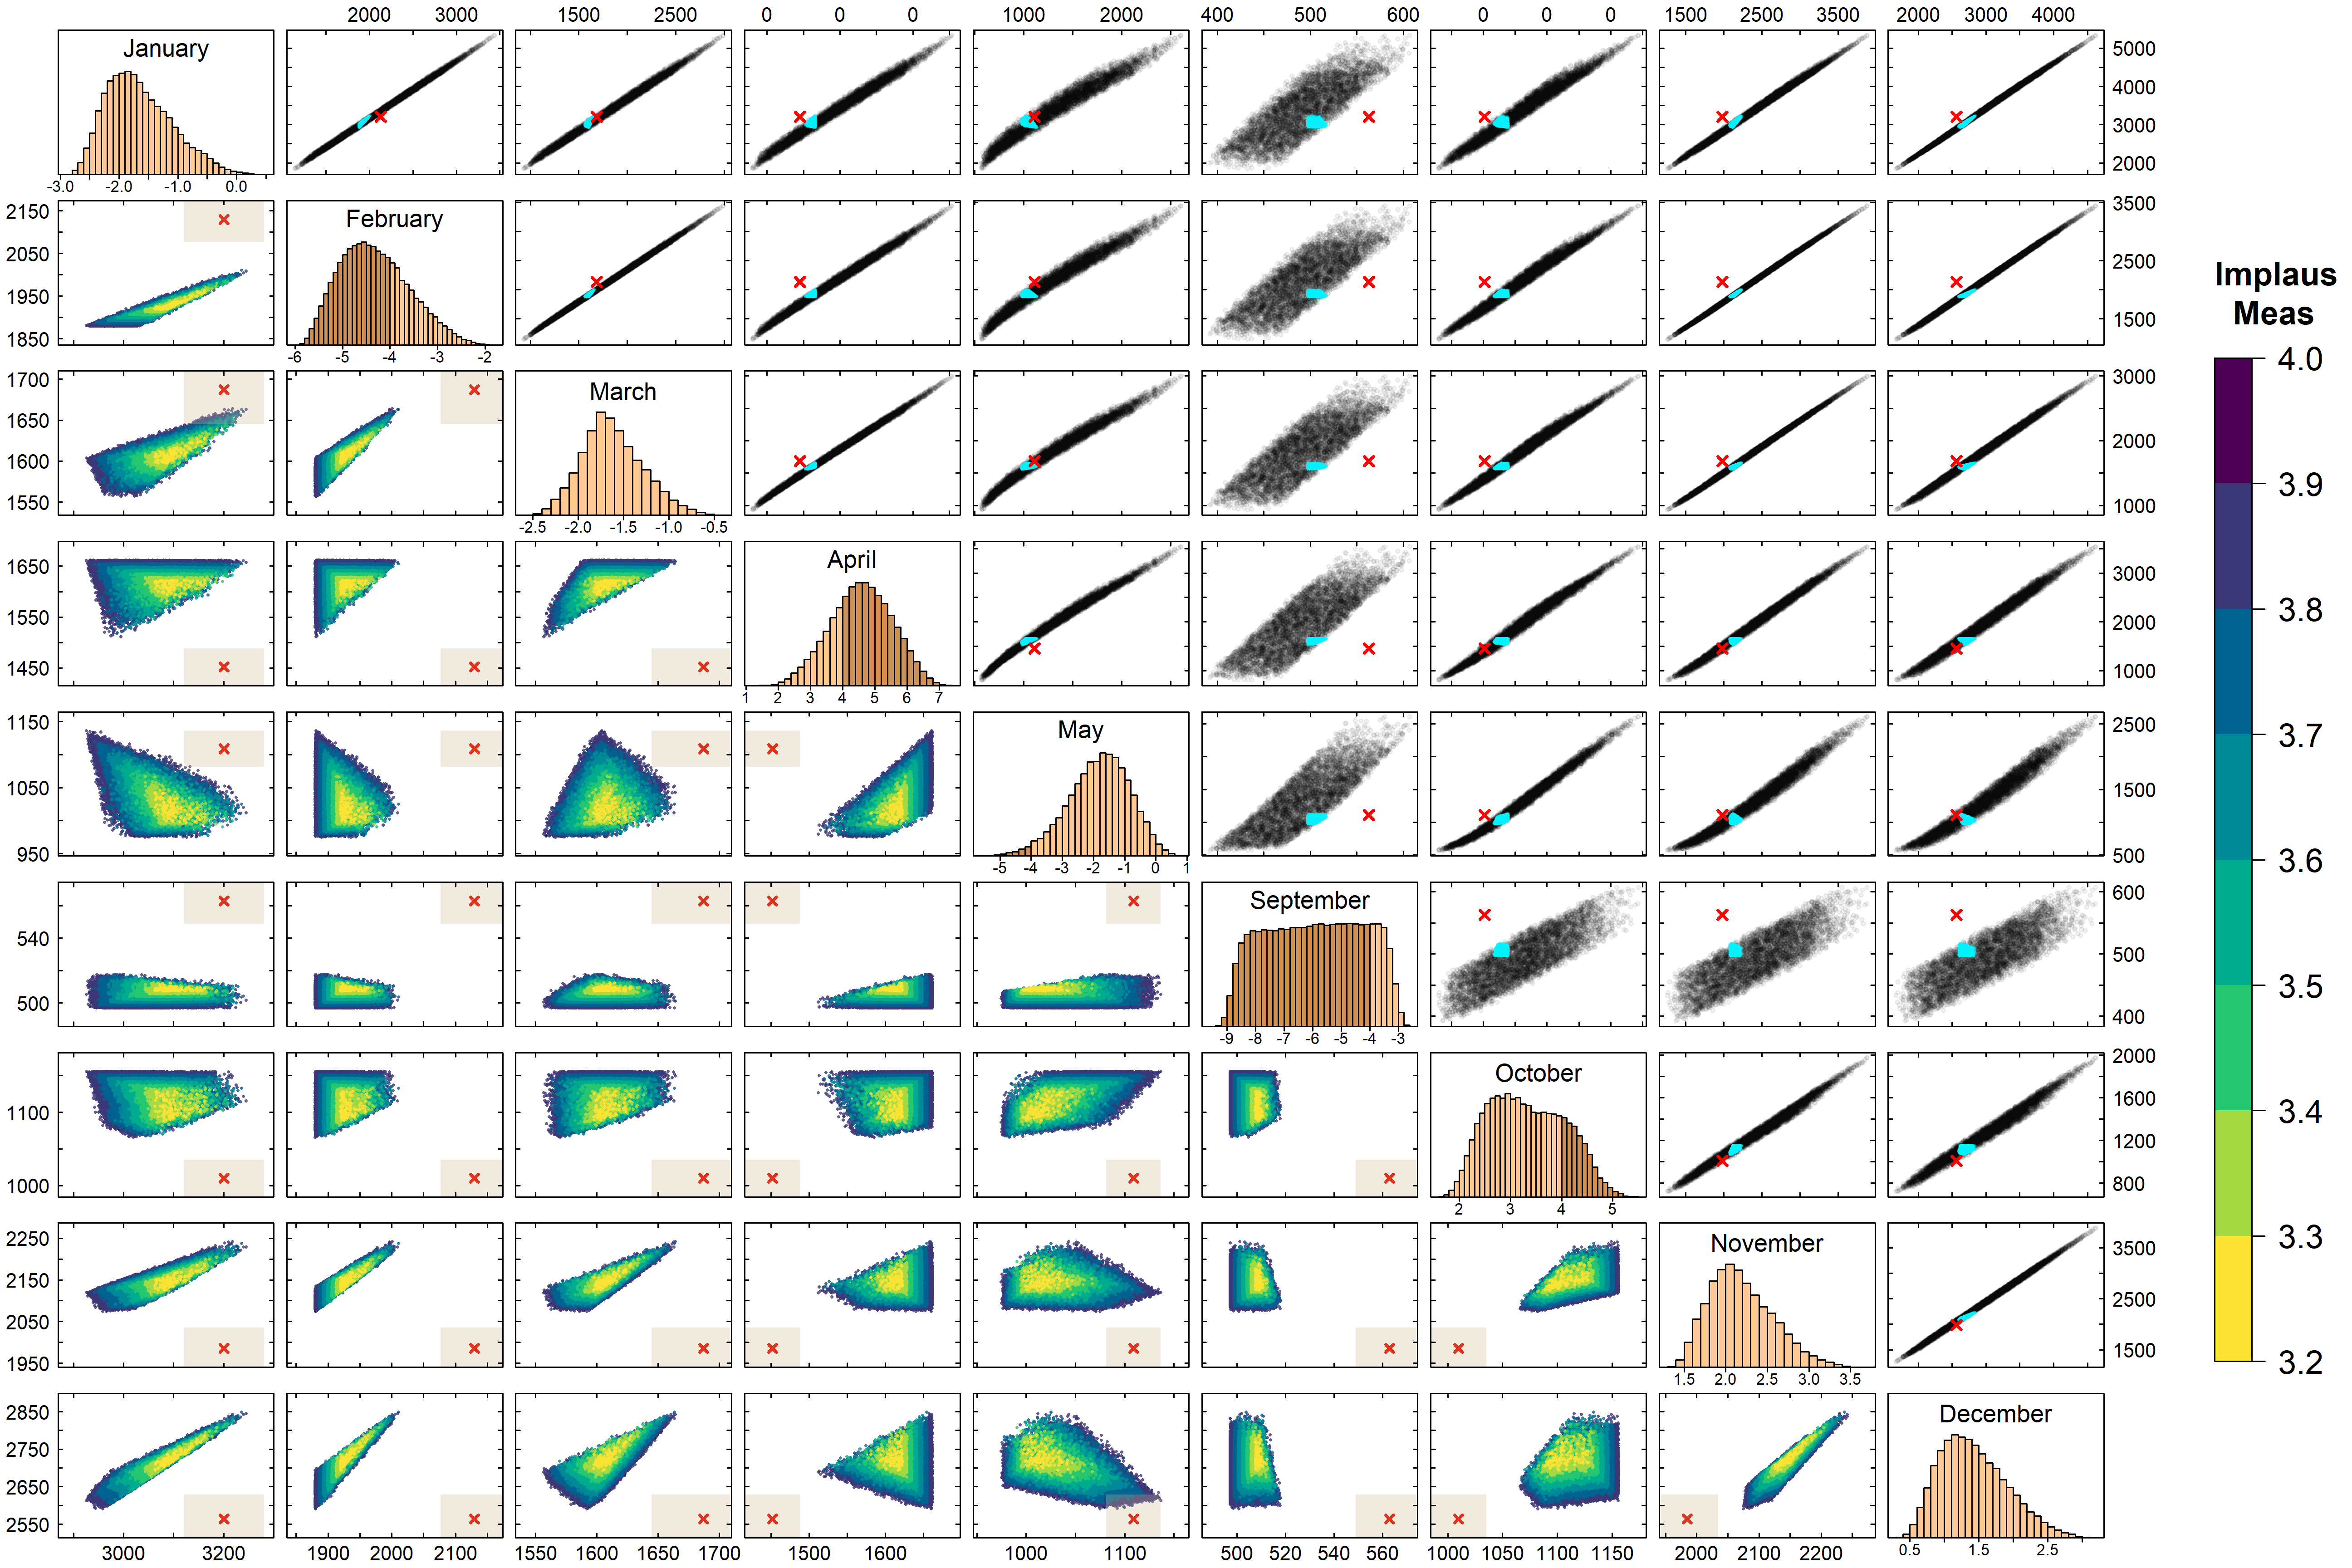
\includegraphics[width=\textwidth]{Non-Implausible_Plots/Gas/Gas_outputs}
\caption{Information on model outputs, observations, and each month’s contribution to cutting the non-implausible region. Upper-diagonal panels: scatter plot of emulated gas consumption for each pair of months (randomly selected 10,000 inputs). The red cross locates the observation to be matched, the light blue stain locates the non-implausible region. Lower-diagonal panels: zoom of the non-implausible region, coloured by implausibility measure (IM). Shaded rectangle around the cross identifies $5\%$ measurement error. Diagonal panels: distribution of each month’s IM, on the space deemed non-implausible when only constraints from the remaining months are considered. The darker colour denotes values outside the interval $[-4,4]$, \textit{i.e.} identifies inputs which transition from being non-implausible to being implausible when that month’s constrain is added. }
\label{Fig_9x9}
\end{figure}

Finally, the histograms on the diagonal of the same figure show the distribution of the IM of a given month, on the points which would be classified as non-implausible if that month was not considered. The IM is reported with its orginal sign (expression~\eqref{eqn_IM} without absolute value), with positive values denoting an emulated consumption higher than the observed one. Values outside the range $[-4,4]$ are highlighted by a darker colour. Months such as January, March, November and December, where all values are between $-4$ and $4$, do not contribute to reduce the space once the other eight months’ constraints are included. On the other hand, a month such as September rules out around $85\%$ of the space that would be considered non-implausible without it.

As the upper-diagonal panels reveal, some of the simulated monthly consumptions are highly correlated, \textit{e.g.}, January’s and February’s. In similar cases, imposing that one month’s observed consumption is matched will limit which observed consumption of the other month can also be matched. In the case of January and February, the location of the cross is very close to the line of simulated consumptions, hence both observations can be easily matched simultaneously (and can also be matched at the same time of all other seven months, as we have seen). However, despite their high correlation, the two months do not play an interchangeable role. The January constraint plays a redundant role the February one is accounted for. But the opposite is not true, as the $x$-range of the two diagonal histograms reveal. The same is true for other pairs of strongly correlated outputs (\textit{e.g.}, Feb-Mar, Feb-Nov, Oct-Nov to a lower extent).

Finally, we notice that many of the lower diagonal projections appear delimited by straight lines. These generally represent the “boundary” beyond which one of the month’s IM exceeds $4$ in absolute value. This is particularly evident for the months whose diagonal histograms extend beyond the interval $[-4,4]$. In this case, the non-implausible region is “cut” perpendicularly to that month’s axis, on the lower or higher side of the range according to whether the histogram exceeds $-4$ or $4$. 


%%%%%%%%%%%%%%%%%%%%%%%%%%%%%%%%%%


\subsection{Adding Temperature Constraints}\label{Subsec_Temperature}

Implausibility measures were previously used to history-match observed gas consumption. They can however be used with any model output for which observations are available, a feature that marks a difference with measures such as MBE and CV(RMSE), as discussed in Section~\ref{Subsec_Limitations}. In our case, we can history match the model temperature predictions in the kitchen and master bedroom, for which hourly time series are available both as observations (field data) and as model outputs. 

Accounting for uncertainty when comparing simulations and observations is more challenging for time series than for scalar quantities. Appropriate tools may involve accounting for correlation across time, dimension-reduction techniques (\textit{e.g.}, PCA) and multidimensional implausibility measures. It is beyond the scope of this work to go into these details, some of which are active areas of statistical research. However, scalar quantities may be extracted from a time series and history-matched through the same methodology discussed in Section~\ref{Sec_Methods}. We show an example here.

In order to include summer constraints, we consider the following scalar quantity: the average temperature difference in July between day (8am--11pm) and night (00am--7am) hours. For each of the two rooms, we compute the above quantity across the $1,000$ design simulations, build an emulator of it as a function of the 8 input parameters, and history-match the parameters.

Notice that the choice of matching temperature difference introduces a different type of constraint to the one imposed on gas, where absolute consumption was matched. We consider the same levels of MD and OE as in Section~\ref{Subsec_OEandMD}. Accounting for each of the two temperature constraints separately rules out as implausible $17.96\%$ (kitchen) and $24.30\%$ (master) of the space respectively (we use here the threshold $T=3$ since only one condition was considered in each of the two cases). Unsurprisingly, we note a strong dependence between the constraints coming from the two rooms: $12.38\%$ of the space is classified non-implausible with respect to both constraints at the same time, which is almost three times more than expected if they were independent.

Accounting for both energy (gas) and environmental (temperature) constraints at the same time classifies only $0.00975\%$ of the original eight-dimensional cube as non-implausible. This is about four times less than it would be expected if the two constraints were independent. The interplay between energy and environmental constraints is highlighted in Fig.~\ref{Fig_Temp}, in the case of three input variables. For each one of them, the plot shows the distribution of non-implausible values for that variable, when the constraints from either gas, or temperature, or both are considered.

As illustration, we comment here on the left plot of Fig.~\ref{Fig_Temp}, which concerns non-implausible values of the heating setpoint (HS) parameter. 

\begin{figure}
\includegraphics[width=\textwidth]{Non-Implausible_Plots/Gas_and_Temperature/Non-Implaus}
\caption{Marginal distribution of three input variables on non-implausible points. The shaded histograms mirror non-implausibility with respect to gas or temperature constraints only, the filled histogram with respect to both.}
\label{Fig_Temp}
\end{figure}

On the one hand, if we only account for the July temperature constraint, the original uniform distribution of heating setpoint values remains unchanged (red shade): this is expected, as heating is switched off in summer and does not, therefore, affect temperature. On the other hand, imposing only the gas constraint shifts the uniform distribution of HS towards the left. However, when both gas and temperature constraints are considered, only higher HS values turn out to be non-implausible. The explanation of this is as follows: third parameters are present whose values are in fact constrained by temperature, and which are correlated with HS. Forcing these parameters to have temperature-compatible values rules out low values of HS. 

Something analogous happens with the boiler efficiency parameter. Finally, the infiltration rate (which plays an important role in limiting temperature oscillation in the building) is indeed mainly driven by the temperature constraint. The additional imposition of the gas constraint only slightly reduces its non-implausible range.


%%%%%%%%%%%%%%%%%%%%%%%%%%%%%%%%%%%%%%%%%%

\section{Conclusion and Extensions of the Work}
\label{Sec_Discussion}

This work has discussed robust ways of accounting for uncertainty in pre-calibration and calibration of building energy models. The methodology has been illustrated on an actual dwelling and its energy model, with the aim of simultaneously matching observations of different nature: energy (gas and electricity use) and environmental (temperature in two zones). 

Our methodology operates in a framework that allows to account for different sources of quantified uncertainty. We have discussed typical sources, such as model discrepancy and measurement error, and shown that their magnitude can play a decisive role in assessing the goodness of a match between simulations and observations. We have therefore illustrated History Matching (HM), a statistical procedure that sequentially rules out regions of the input space where simulations cannot match observations. 

To explore the model’s response throughout the input space, HM makes use of statistical emulators. Once built and validated, an emulator only requires milliseconds on a personal laptop to predict the model response on a new input configuration, and its prediction uncertainty can be naturally embedded in the HM framework. The hmer R package allows to implement emulation and the whole HM procedure \cite{hmer}.

While HM generally proceeds in multiple waves, in the example study discussed in this work one wave was enough to identify the final non-implausible region. This is a peculiarity of this example, where remarkably precise emulators for all quantities of interest could be built over the whole input space. In general, one of the strengths of HM is that the above is not at all required. Some of the outputs may not even be emulated in early stages. The sequential procedure allows the researcher to add constraints as the procedure moves to later waves. A quantity that was difficult to emulate in a given wave often behaves more smoothly within the more constrained NROY region of a later wave, and it can therefore be emulated with great precision at that stage. 

Also notice that in our case, the speed of the E+ model allowed us to run $1,000$ simulations initially. Such a large number of runs is, once again, not needed in general. In fact, HM only needs a few runs at the start. The procedure itself will guide the researcher to focus new simulations within a sequence of smaller regions, that eventually converge to the final non-implausible region. In additiona experiments that has not been detailed in this work , we have randomly selected 100 of the original $1,000$ simulations and used these to train (80 runs) and validate (20 runs) the new emulators. However, the quadratic behaviour of the simulator was easily captured by the 80 simulations, yielding results that, after only one wave of HM, were practically identical to the ones shown in Section~\ref{Sec_Results}, where all $1,000$ simulations were used.

Whilst emulators are classically used as model surrogates in HM, it is worth observing that less precise surrogates of the model may also be used (\textit{e.g.}, linear regression), especially during the first explorative stages of research. Using linear regression, for example, would only take a few minutes of computational power but still allows the researcher to get a feeling of where the non-implausible region lies, while operating in a sound uncertainty framework.

In terms of computational power, the efficiency of emulation over the original simulator is apparent. All emulation and HM computations carried out in this work were performed on a personal laptop with 16GB RAM and 1.9GHz processor. For gas, and without any parallelisation, the computations (emulation and HM at $10^7$ inputs, for nine months) were carried out in less than 28 hours. While still several orders of magnitude faster than the model running times, this is relatively slow for emulation standards, due to the high number of training points used (700). With only 80 training points, the same computations on the same device are executed in 2h and 5min. If we were to use the original E+ simulator directly, $10^7$ simulations would have instead required about 18 years (as our original $1,000$ simulations were performed in about 16 hrs).

Finally, extensions of the methodology illustrated here can be manifold. Suppose a simulator is exceptionally slow to run, and faster versions produce lower-resolution results. A Bayesian framework where accurate emulators of the expensive model can be built, by using results of the faster version as prior information, is illustrated in \cite{cumming2009}. This approach is referred to as multi-level (or multi-fidelity) emulation; an application for transport of volcanic ashes is discussed in \cite{harvey2018}. Applications in the energy sector may concern the case of multi-vector energy modelling across districts or even national level, which is becoming crucial as a diverse mix of renewable inputs are used to replace fossil-based alternatives. Another similar example is building fabric energy modelling at building, cluster or even urban level whereby increasing the physical boundary and resolution of the model imposes a very heavy computational duty.   

An additional extension of the methodology we have discussed concerns the HM of time series data. This requires the use of emulators for time-evolving systems, as discussed for example in \cite{conti2009}. Multivariate implausibility measures (\cite{vernon2010galaxy, cumming2010}) may then be used to assess the distance between predicted and observed time series. This however requires a thoughtful specification of the time-correlation not only for the time series in question, but also for MD and OE. A discussion of this is beyond the scope of this work, but the interested researcher may refer to [ref]  for an example of application to ***.\red{(Michael, Hailiang, suggestion here?)}




%%%%%%%%%%%%%%%%%%%%%%%%%%%%%%%%%%%%%%%%%%
%% The Appendices part is started with the command \appendix;
%% appendix sections are then done as normal sections
%% \appendix

\bibliographystyle{elsarticle-num} 
\bibliography{References}


\end{document}
\endinput
%%
%% End of file `elsarticle-template-num.tex'.
